\lhead{\begin{tikzpicture}[remember picture, overlay]
\node [anchor=100,inner sep=0] (imagenIZQUIERDA) at (current page header area.north){
\includegraphics[width=18cm]{img/Encabezado.PNG}};
\end{tikzpicture}}
\rhead{Piedra-Moreno}
\rfoot{\begin{tikzpicture}[remember picture, overlay]
\node [anchor=140,inner sep=0] (imagenDERECHA) at (current page footer area.south){
\includegraphics[width=18cm]{img/Foot.PNG}};
\end{tikzpicture}}
%----------------------------------------------------------------------------------------
\lfoot{ \thepage}
% \renewcommand{\labelenumi}{\alph{enumi}.)} 
%----------------------------------------------------------------------------------------
%----------------------------------------------------------------------------------------
%	TITLE SECTION
%----------------------------------------------------------------------------------------

\setlength{\droptitle}{-5\baselineskip} % Move the title up
\title{\textbf{Estudio de tiempos y movimientos en el ensamble de un circuito electrónico utilizando diferentes métodos para su optimización }} % Article title

 \author{ 
 \textsc{Piedra-Moreno, Alitza Alejandra}\\ 
 \texttt{ Instituto Tecnológico de Querétaro } \\ 
 \texttt{ Tecnológico Nacional de México } \\ 
 \texttt{Querétaro, México}\\ 
 \texttt{l22140912@queretaro.tecnm.mx} 
 \and 
 \textsc{Ángeles-Hurtado, Luis Alberto}\\ 
%  Afiliación:
 \texttt{ Instituto Tecnológico de Querétaro } \\ 
 \texttt{ Tecnológico Nacional de México } \\ 
 \texttt{Querétaro, México}\\ 
 \texttt{alb3rt0.ah@gmail.com} 
}


%----------------------------------------------------------------------------------------

% \begin{document}

% Print the title
\maketitle
\thispagestyle{fancy}

%----------------------------------------------------------------------------------------
%	ARTICLE CONTENTS
%----------------------------------------------------------------------------------------

% \section*{Resumen}
% \textit{Palabras clave:}
% El resumen (ancho de página) deberá contener entre 100 y 200 palabras tipo Adobe Devangari 11 puntos.

\begin{abstract}
\noindent 
El resumen (ancho de página) deberá contener entre 100 y 200 palabras tipo Adobe Devangari 11 puntos.

\end{abstract}
% 
% 
\textbf{\textit{Palabras clave}}: {Estudio, análisis, tiempo, movimiento, estándar, empresa, industrial, operación, muestra}
% \keywords{First keyword should be the corresponding to the research area according with the authors guide. Maximum of 6 keywords.}

\section{Introducción}

% Define estudio de tiempos y movimientos
% define que es ensamble
% define que es circuito electronico
% define el metodo de tiempos predeterminados
% define optimización
\begin{itemize}
    \item Se debe exponer de manera concreta y en lenguaje sencillo: el tema, o lo(s) objeto (s) de estudio. 
    \item Se deben de mencionar las metodologías más usadas muy brevemente. 
    \item Se debe de señalar el avance en los últimos años.
    \item Al final se debe hacer alusión al o lo(s) objetivos del proyecto de investigación.
    \item Debe de tener Referencias científicas, URL, tesis, etc.
\end{itemize}


¿Se sabe como es que funciona el método actual del ensamblaje del circuito electrónico? ¿Conocemos el porqué de este método? ¿Podemos mejorar este método? ¿Existe una forma más economía y óptima para realizar el trabajo?

El estudio de movimientos y tiempos, se define el análisis de los movimientos, herramientas, materiales, e instalaciones utilizadas y que se han de utilizar, teniendo como meta encuentra la forma más económica de realizar el trabajo, normalizar los métodos, materiales, herramientas e instalaciones, determinar el tiempo estándar y ayudar al aprendizaje de los métodos. En la actualidad las empresas u organizaciones, sin importar su tamaño e industria, enfrentan enormes desafíos que les exigen ser competitivas en el mercado globalizado, la productividad de las empresas se ve más afectada por la distribución y relaciones de las plantas, entre diferentes sectores empresariales. Las empresas buscan la mejor manera de integrar herramientas basadas en estudios de métodos y medición de procesos utilizando observación directa y secuencial de procesos, determinando diagramas de flujo, tiempos, distancias, actividades, funciones, tiempos de inactividad, expectativas, almacenamiento, transporte, aquí se toman referencias para comparar, decidir e implementar cambios y tendencias para aumentar la eficiencia de la producción.

Como para todo, el desarrollo de un estudio del trabajo tiene un procedimiento o se secuencian de pasos, la cual se debe seguir y se muestra a continuación: 


 \begin{enumerate}
     \item Seleccionar el trabajo o proceso a estudiar. 
     \item Registrar  y  organizar  la  información  disponible,  utilizando  las técnicas apropiadas para tal fin. 
     \item Analizar las situaciones encontradas críticamente,  preguntándose si se justifica lo que se hace, según el propósito de la actividad. 
     \item Definir el  lugar en donde  se llevará a  cabo, establecer el  orden de ejecución. 
     \item Definir el responsable de la ejecución del procedimiento y los medios a  emplear,  utilizando  el  método  más  económico  para  todas  las circunstancias.
     \item Medir la cantidad de trabajo que exige el método elegido y calcular el tiempo tipo que lleva hacerlo.
     \item Definir el nuevo método y el tiempo correspondiente para que pueda ser identificado en todo momento. 
     \item Implementar el nuevo método  como práctica general aceptada  con el tiempo fijado. 
     \item Mantener  en  uso  la  nueva  práctica mediante  procedimientos  de control adecuados \cite{niebel1980ingenieria}
 \end{enumerate}

Como se puede observar estos son solo unos de los pasos que se deben seguir para realizar nuestro estudio, dentro de ellos podemos decir que a la hora del análisis uno debe desglosar la operación en elementos y entre estos debemos incluir los Therblings, los cuales están divididos en eficientes e ineficientes y en los cuales nuestro trabajo es eliminar la mayor parte de los ineficientes, disminuir los eficientes e identificar cada uno de estos en los pasos a realizar. Como consecuencia, para lograr este objetivo, debemos utilizar los métodos de medición del tiempo, es un sistema estandarizado para medir los tiempos que tardan los operadores en realizar una tarea repetitiva, esto con el objetivo anteriormente mencionado de analizar donde se encuentran los movimientos ineficientes, que son sinónimos de perdidas innecesarias \cite{DanielGrifol}

Para ello mismo, en el proyecto se debe generar un método de muestreo, donde se escogerá las muestras más representativas que sean de calidad, que describan de manera exacta las características de un conjunto de que nos permitan predecir, deducir, inferir y sacar conclusiones de este ensamble, y lograr ser lo más exacto y preciso posible. Con esto en cuenta se utilizará lo que se conoce como muestreo de trabajo, la cual nos sirve para disminuir los costos que presenta un estudio continuo del tiempo o estudio de tiempos convencional, el cual implica un esfuerzo y trabajo mayor.

con el motivo de generar una precisión más exacta se utilizará el tiempo productivo el cual es la calificación del desempeño del operador, basándonos en la experiencia, capacitación, y juicio del analista, esto con motivo de normalizar y estabilizar los tiempos generando un intervalo de tiempos menor, reduciendo así el intervalo de confianza. Con esto en mente tenemos el objetivo de realizar estas muestras, para poder deducir lo que es el tiempo ciclo y estándar a través de lo que es la probabilidad y estadística con la cual nos centraremos en o que es el método del límite central para generar una media que nos ayudara a ser más exactos en el tiempo estándar de nuestra operación, ayudándonos a tener una visión más clara de nuestras bases para posteriormente generar una mejora, en el método, materiales, distribución y hasta instalaciones.

\subsection{Definiciones}

\subsubsection{Latex}

LaTeX es un sistema de composición de textos, orientado especialmente a la creación de libros, documentos científicos y técnicos que contengan fórmulas matemáticas.

LaTeX está formado por un gran conjunto de macros de TeX, escrito por Leslie Lamport en 1984, con la intención de facilitar el uso del lenguaje de composición tipográfica, TeX. Es muy utilizado para la composición de artículos académicos, tesis y libros técnicos, dado que la calidad tipográfica de los documentos realizados con LaTeX es comparable a la de una editorial científica de primera línea.
\cite{Dlsi.ua.es}

\subsubsection{Github}

GitHub es una plataforma de alojamiento, propiedad de Microsoft, que ofrece a los desarrolladores la posibilidad de crear repositorios de código y guardarlos en la nube de forma segura, usando un sistema de control de versiones llamado Git.

Facilita la organización de proyectos y permite la colaboración de varios desarrolladores en tiempo real. Es decir, nos permite centralizar el contenido del repositorio para poder colaborar con los otros miembros de nuestra organización.
\cite{Platzi}

\subsubsection{Git}

Git es un sistema de control de versiones distribuido, lo que significa que un clon local del proyecto es un repositorio de control de versiones completo. Estos repositorios locales plenamente funcionales permiten trabajar sin conexión o de forma remota con facilidad.

\cite{Microsoft}

\subsubsection{Visual studio code}

Visual Studio Code (VS Code) es un editor de código fuente desarrollado por Microsoft. Es software libre y multiplataforma, está disponible para Windows, GNU/Linux y macOS. VS Code tiene una buena integración con Git, cuenta con soporte para depuración de código, y dispone de un sinnúmero de extensiones, que básicamente te da la posibilidad de escribir y ejecutar código en cualquier lenguaje de programación.\cite{OpenWebinars.net}

\subsubsection{Estudio de movimientos}

Implica el análisis cuidadoso de cada uno de los movimientos corporales que se emplean para realizar una tarea. 
\cite{niebel1980ingenieria}
Es el análisis de métodos, materiales, herramientas, e instalación utilizada o que se ha de utilizar en la ejecución de un trabajo.

\subsubsection{Movimientos básicos} 
Como parte del análisis de movimientos, los Gilbreth concluyeron que todo trabajo, ya sea productivo o no, se realiza mediante el uso de combinaciones de 17 movimientos básicos a los que ellos llamaron therblig \cite{niebel1980ingenieria}  

Estos se dividen en eficientes, que estimulan el progreso del trabajo y con frecuencia pueden ser acortados, pero por lo general no pueden ser eliminados:
\begin{enumerate}
    \item \textbf{Alcanzar (AL):} “Mover” la mano vacía hacia o desde el objeto; donde el tiempo depende de la distancia recorrida.
    \item \textbf{Mover (M):} “Mover” la mano cargada; el tiempo depende de la distancia, el peso y el tipo de movimiento.
    \item \textbf{Tomar (T):} “Cerrar” los dedos alrededor de un objeto, este comienza cuando los dedos tocan el objeto y termina cuando se ha ganado el control.
    \item \textbf{Soltar (SL):} “Soltar” el control de un objeto, normalmente el más corto de los therbligs.
    \item \textbf{Preposicionar (PP):} ”Posicionar” un objeto en una ubicación predeterminada para su uso posterior. Por lo general ocurre en conjunto con “Mover”.
    \item \textbf{Utilizar (U):} “Manipular” Una herramienta para el uso por el que fue diseñada; fácilmente detectable a medida que avanza el progreso del trabajo.
    \item \textbf{Ensamblar (E):} “Unir” dos partes que embonan. Por lo general es precedido por “Posicionar” o “Mover” y seguido por “Liberar”.
	\item \textbf{Desensamblar (DE):} Es lo opuesto a “Ensamblar”, pues separa partes que embonan.

 También encontramos los ineficientes, los cuales no representan un avance en el proceso del trabajo y debe eliminarse. En esta categoría encontraremos:

    \item \textbf{Buscar (B):} Ojos o manos buscan un objeto; comienza a medida que los ojos se mueven para localizar un objeto.
    \item \textbf{Seleccionar (SE):} “Mover” la mano cargada; el tiempo depende de la distancia. Por lo general es seguido por “Buscar”.
    \item \textbf{Sostener (SO):} Una mano soporta el objeto mientras la otra realiza trabajo útil.
    \item \textbf{Posicionar (P):} “Orientar” un objeto durante el trabajo, por lo general precedido por “Mover” y seguido por “liberar”.
    \item \textbf{Inspeccionar (I):} “Comparar” un objeto con el estándar, típicamente a la vista, pero podría ser también con los demás sentidos.
    \item \textbf{Planear (PL):} “Pausar” para determinar la acción siguiente; por lo general se le detecta como un titubeo que precede a “Mover”
    \item \textbf{Retraso Inevitable (DI):} Más allá del control de quien opera debido a la naturaleza de la operación.
    \item \textbf{Retraso Evitable (DEV):} Quien opera es único/a responsable del tiempo ocio.
    \item \textbf{Descansar (DES):} Aparece periódicamente, no en cada ciclo. Depende de la carga de trabajo física.

\end{enumerate}

\subsubsection{Sistemas de tiempo predeterminado}

Conjunto de reglas o métodos para determinar con anticipación la secuencia de sucesos.

\subsubsection{Métodos de medición del tiempo}

 Es un sistema estandarizado para medir los tiempos que tardan los trabajadores en ejecutar una tarea repetitiva. El objetivo de este sistema es analizar donde están los movimientos ineficaces que se traducen en pérdidas innecesarias de tiempo en una tarea que se ejecuta cientos de veces al día. \cite{DanielGrifol}

\subsubsection{Precisión}

La precisión es lograr la mínima dispersión al momento de hacer una medición o de realizar una tarea. Es la variación o poca variación significa un buen grado de precisión.

\subsubsection{Exactitud}

Se define con respecto a su cercanía o sesgo, mayor cercanía implica un buen grado de exactitud.

\subsubsection{Muestreo}

Acción de escoger muestras representativas de calidad que describa de manera exacta las características de un conjunto que nos dejen deducir, inferir y sacar conclusiones de un fenómeno a estudiar. \cite{RAE}

\subsubsection{Representativo}

Significativo, característico, peculiar, relevante e importante. \cite{RAE}

\subsubsection{Inferir}

Deducir algo o sacarlo de conclusión de otra cosa.\cite{RAE}

\subsubsection{Muestreo de trabajo}

Lo podemos considerar como una herramienta para disminuir el costo que se presenta  en el estudio continuo del tiempo. Su único problema es obtener una muestra representativa.

\subsubsection{Estudio de tiempos convencional}

Es una muestra continua de n ciclos suponiendo que la distribución estadística es normal.

\subsubsection{Estudio de tiempos no convencional}

Esta contiene huecos entre las lecturas de muestreo y es una muestra discreta suponiendo que la distribución estadística es binomial.

\subsubsection{Tiempo productivo}

El tiempo productivo es la calificación del desempeño de operador, está basada en la experiencia, capacitación y juicio del analista que lo realiza.

\subsubsection{Diagrama de procesos de bimanual}

Herramienta que muestra todos los movimientos y retrasos atribuibles a las manos derecha e izquierda, además de la relación que existe entre ellas. 
Tiene como propósito identificar los patrones de movimiento que resultan ineficientes y observar las violaciones a los principios de la economía de movimientos.\cite{niebel1980ingenieria}

\subsubsection{Colocación de las herramientas y materiales}

En cada movimiento que se realiza está involucrada una distancia, a medida que la distancia es mayor, el esfuerzo muscular, el control y el tiempo serán mayores. Por ello, minimizar las distancias es lo que se busca.

El área de trabajo normal en el plano horizontal de la mano tanto derecha e izquierda incluye el área circunscrita por el brazo bajo el codo cuando se mueve para formar un arco que gira con respecto al codo.

Esta representa la zona más conveniente dentro de la cual es más cómodo realizar movimientos con la mano y no consumirá más energía de la requerida. El área máxima es la zona que  comprende un movimiento más amplio de los brazos, es decir, el área virtual que abarcan los brazos al hacer un “barrido” y completamente extendidos. Entendiendo que el área máxima será para aquellos elementos que se usan con una frecuencia menor, en un promedio de 3 veces por hora, pues esta zona depende de un movimiento más amplio. \cite{niebel1980ingenieria}

\subsubsection{Equipo para el estudio de tiempos}

El equipo mínimo requerido para realizar un programa de estudio de tiempos incluye un cronómetro, un tablero de estudio de tiempos, las formas para el estudio y una calculadora de bolsillo. Un equipo de videograbación también puede ser muy útil.

\textbf{Cronometro}
Reloj de gran precisión para medir fracciones de tiempo muy pequeñas, utilizado en industria y en competiciones deportivas.
\cite{RAE}

\textbf{Cámaras de videograbación}
Las cámaras de videograbación son ideales para grabar los métodos del operario y el tiempo transcurrido. Al tomar película de la operación y después estudiarla cuadro por cuadro, los analistas pueden registrar los detalles exactos del método usado y después asignar valores de tiempos normales. 

\textbf{Tablero de estudio de tiempos}

Los analistas encuentran conveniente tener un tablero adecuado para sostener el estudio de tiempos y el cronómetro. El tablero debe ser ligero, fuerte y suficientemente duro para proporcionar el apoyo necesario para la forma de estudio de tiempos. El tablero debe tener contactos para el brazo y el cuerpo con el propósito de que el ajuste sea cómodo y resulte fácil escribir mientras se sostiene.

\textbf{Forma de estudio de tiempo}

En una forma de estudios se registra toda la información pertinente sobre el método que se estudia, las herramientas utilizadas, etc. La operación en estudio se identifica mediante información como nombre y número del operario, descripción y número de la operación, nombre y número de la máquina, herramientas especiales usadas y sus números respectivos, el departamento donde se realiza la operación y las condiciones de trabajo prevalecientes. 
\cite{niebel1980ingenieria}

\subsubsection{Ciclos en el estudio}
 Como el estudio de tiempos es un procedimiento de muestreo, se puede suponer que las observaciones se distribuyen normalmente respecto a una media poblacional desconocida con una varianza desconocida. Si se usa la media muestral y la desviación estándar muestral s, la distribución normal para una muestra grande lleva al siguiente intervalo de confianza.

\begin{equation}
    \label{eq1}
    x {\pm} {\frac{zs}{\sqrt{n}}}
\end{equation}

\subsection{Teorema}
Proposición demostrable lógicamente partiendo de axiomas, postulados o de otras proposiciones ya demostradas.\cite{RAE}

\subsection{Preposición}
Expresión de un juicio entre dos términos, sujeto y predicado, que afirma o niega este de aquel, o incluye o excluye el primero respecto del segundo. \cite{RAE}

\subsection{Axioma}
Proposición tan clara y evidente que se admite sin demostración.\cite{RAE}

\subsection{Postulado}
 Idea o principio sustentado por una persona, un grupo, una organización, etc. Proposición cuya verdad se admite sin pruebas para servir de base en ulteriores razonamientos.\cite{RAE}
 
\subsection{Límite}
 En una secuencia infinita de magnitudes, magnitud fija a la que se aproximan cada vez más los términos de la secuencia. Así, la secuencia de los números 
 
\begin{equation}
\label{eq1}
    {\frac{2n}{n+1}}
\end{equation}
, siendo n la serie de los números naturales, tiene como límite el número 2.\cite{RAE}


\subsection{Límite inferior}
En un conjunto de magnitudes, magnitud máxima que es inferior a todas las del conjunto.\cite{RAE}

\subsection{Límite superior} 

En un conjunto de magnitudes, magnitud mínima que es superior a todas las del conjunto. \cite{RAE}

\subsection{Teorema de límite central}



\section{Justificación}

La industria constituye la actividad más importante de la producción material en la mayoría de los países. Tal y como se conoce hoy, esta actividad se desarrolla a partir de la revolución industrial en Inglaterra y ha estado estrechamente ligada al progreso en los países capitalistas más avanzados.

Durante la mayor parte de la centuria pasada, los economistas llegaron a establecer una conexión directa entre industrialización y desarrollo, fundamentalmente sobre la base de la experiencia de los países ricos y, luego, de la extinta Unión de Repúblicas Socialistas Soviéticas (URSS). Varios economistas destacados, como Rosenstein-Rodan (1943), Prebisch (1950), Lewis (1954), Hirschman (1958) y otros, le otorgaron un lugar central a la manufactura en el esfuerzo de desarrollo de los países más atrasados. Su valor se relacionó con la explotación de economías de escala junto a una alta y creciente productividad del trabajo; su papel, con la mejoría de los términos de intercambio, el acelerado cambio técnico y una gran capacidad de impactar en el avance de otras ramas a través de encadenamientos productivos. Kaldor (1966), por ejemplo, resaltó que estos elementos permitían explicar la presencia de rendimientos crecientes, lo que estaría detrás del colapso del crecimiento económico en estados industrializados que experimentaran una pérdida sostenida de su tejido industrial. 



La mayoría de estos efectos se han manifestado claramente en la trayectoria de un grupo de nuevos países industrializados (NPI), esencialmente en Asia, pero también en el caso de Irlanda y Brasil. Un aspecto especialmente relevante tiene que ver con su impacto en el avance científico-técnico y en la innovación-desarrollo (I+D). Datos recientes (McKinsey Global Institute –MGI–, 2012) indican que más del 90 \% del gasto en I+D en el sector productivo se origina en la manufactura; mientras que las cinco revoluciones tecnológicas descritas hasta la actualidad (Pérez, 2002) han tenido como punto de partida la actividad industrial, para luego generar considerables externalidades hacia el conjunto del sistema económico.

Estas consideraciones forman parte de la agenda de desarrollo para las naciones pobres y, por supuesto, también para Cuba. Por ello es indispensable conocer las tendencias más importantes del desarrollo industrial en el mundo y sus consecuencias para la formulación de políticas en este grupo de estados

    En la actualidad, la competitividad de las empresas es considerada una cuestión fundamental en los sectores económicos tanto de los países desarrollados como en desarrollo. El contexto internacional y en especial el proceso de globalización requieren que las organizaciones cuenten con recursos eficaces y eficientes en la gestión de los recursos financieros, humanos, naturales y tecnológicos, entre otros, para afrontar el desafío del mercado, no solo nacional, sino fuera de las fronteras de sus países de origen. \cite{labarca2007consideraciones}
    
    En el nivel medio o marco, la competitividad está relacionada con las ventajas relativas de los recursos de un país o región, ya sea tierra, trabajo y capital, o con las ventajas que surgen principalmente de las inversiones en formación de capital humano e innovación. \cite{padilla2006instrumento}
    
    En la situación actual, donde prevalecen continuos y rápidos cambios tecnológicos, la formación juega un papel muy importante para fortalecer la competitividad de la empresa, como productora de capital humano. Por un lado, complementa la formación formal, proporcionando al empleado los conocimientos y habilidades necesarios para utilizar, adaptar y, en última instancia, mejorar la tecnología. Por otro lado, dado que tiene como objetivo proporcionar a los empleados los conocimientos y habilidades que necesitan en sus operaciones diarias, se puede esperar que genere un retorno rápido y significativo para la empresa.\cite{casar1993competitividad}
    
    Desde comienzos de año, diversos indicadores muestran una clara divergencia entre la actividad del sector manufacturero y el sector servicios. De hecho, según los índices PMI globales, la actividad manufacturera se está enfriando desde inicios del pasado año (y se encuentra ya estancada o en retroceso en algunos países), mientras que el sector servicios ha mostrado una notable recuperación.
    
    Parte de esta divergencia entre manufacturas y servicios responde a su diferente naturaleza cíclica. El consumo de bienes duraderos y la producción manufacturera son muy cíclicos y sensibles a cambios en las condiciones monetarias. Por tanto, es lógico pensar que la notable tensión experimentada por las condiciones monetarias globales desde comienzos de 2022 ha terminado enfriando la actividad en el sector industrial. Sin embargo, existen otros motivos que explican que la discrepancia sectorial actual se encuentre en máximos desde la crisis financiera de 2008. \cite{CaixaBank}
    
    Querétaro es uno de los estados con el mayor número de parques industriales del país, donde están asentadas empresas mexicanas, estadounidenses, alemanas, canadienses y coreanas.
    
    El sector industrial en el estado de Querétaro, aporta el 36 por ciento de los empleos totales en la entidad. Es decir, hay 352 mil puestos laborales en este sector.Esto debido a que se tiene un total de 49 parques industriales en la entidad.
    
    Querétaro se ha destacado a lo largo de los años por su notable crecimiento económico y por mantenerse en los primeros lugares dentro de los indicadores de actividad económica. Este significativo desarrollo económico e industrial se refleja en que Querétaro es de los estados con mayor número de parques industriales del país. \cite{JessicaIgnot}
    
    En el estado se tiene registro de 67 parques y zonas industriales, que se concentran principalmente en El Marqués (34.3\%), Querétaro (31.1\%), Colón (13.4\%); los restantes están en Pedro Escobedo, Huimilpan, Corregidora y Cadereyta (20.9\%), expone el Anuario Económico Estatal, edición 2021, de la Secretaría de Desarrollo Sustentable (Sedesu).



% 
% 
\section{Descripción del problema}
\begin{itemize}
    \item Se debe describir la desviación o diferencia del ``es'' con respecto al ``debe ser''.
    \item Se debe hacer alusión a la incógnita científica*.
    \item Debe de tener Referencias científicas, URL, tesis, etc.
\end{itemize}

\textbf{*La incógnita científica es el elemento cuya solución incrementa el conocimiento científico.}
% 
% 
\section{Fundamentación teórica}

Es la parte medular y de mayor discusión, deberá ser la fundamentación de la hipótesis, por tanto, se deberá señalar claramente la razón de la suposición y fundamentación de la misma. Únicamente referencias científicas.
\begin{itemize}
    \item Se debe de retomar el tema que se planteó en la introducción, pero ahora profundizando para clarificar la incógnita científica y se pueda plantear la hipótesis.
    \item Se debe de retomar la descripción del problema, pero ahora en profundidad del (los) objeto(s) de estudio. 
    \item Se debe de profundizar en las metodologías que se ha usado para el estudio del tema.
    \item Referencias solo de artículos y libros científicos.
\end{itemize}
% 
% 
\section{Hipótesis}

Es la suposición con fundamento científico relativa a la solución del problema, necesidad o de cómo se aprovecha la oportunidad con la incógnita científica y se fundamenta con: 1. Una suposición (en afirmativo o negativo) y esta deberá vincularse con:
2. La fundamentación científica que deberá ser precisa 3. Una entidad de comparación para probar la suposición y
4. La variable con que se califica o cuantifica la comparación o se prueba la hipótesis.

\begin{itemize}
    \item Se debe de identificar claramente la suposición científica
    \item Se debe de identificar claramente el fundamento científico
    \item Se debe identificar claramente la variable de respuesta
    \item Se debe identifican claramente las realidades o modelos contrastantes
    \item Se debe de establecer las variables asociadas, explicativas o que tienen relación funcional con la variable de respuesta
\end{itemize}
% 
% 
\section{Objetivo}

Diseñar, mejorar e integrar sistemas productivos de bienes aplicando tecnologías para su optimización. Diseñar, implementar y mejorar sistemas de trabajo para evaluar la productividad. Analizar, los movimientos, herramientas, materiales e instalaciones utilizadas y que se han de utilizar para encontrar la forma más económica de hacer, el trabajo. Normalizar los métodos, materiales, herramientas e instalaciones, usadas. Determinar el tiempo necesario y estándar de realización del trabajo.


\subsection{Objetivos específicos}

\begin{itemize}
    \item Identificar los materiales, describirlos, recaudar información de ellos, estandarizarlos y normalizarlos.
    \item Crear una secuencia de pasos para estandarizar los procedimientos a realizar en el ensamblaje.
    \item Dividir las operaciones en elementos, para posterior identificar y eliminar los movimientos ineficientes.
    \item Generar un muestro de calidad, y que sea representativo para la toma de tiempos.
    \item Conseguir el tiempo siclo.
    \item Obtener la media muestral y la desviación estándar para estimar lo que es conocido como la media poblacional y la variancia.
    \item Obtener una aproximación al tiempo estándar de la operación.
    
\end{itemize}

% 
% \section{Cuerpo }

\section{Metodología}

\subsection{Instructivo}

En la figura \ref{fig:Distribucion inicial }se muestra la distribución propuesta para la primera parte del análisis donde aún es con el método actual, lo cual es indispensable para notar los cambias y por ello mismo el operario debe asegurar que esta distribución se cumpla a la hora de realizar la operación.
    \begin{figure}[H]
    \centering
    \includegraphics[trim = {20mm 10mm 7mm 10mm},clip,scale=0.35]{22/Img/ensamblaje.pdf}
    \caption{Distribución inicial}
    \label{fig:Distribucion inicial}
\end{figure}
    
\begin{enumerate}

    \item Posiciona el protoboard en el área de ensamblaje.

    \item Coloca la ESP32 en el centro del protoboard colocando los pines NC en la columna 30 y en las filas B e I de forma que el pin 3V3 esté en el punto 15-B y quede simétrico, dejando la fila a y j libres. 

    \item Conecta un cable MM (azul) en el punto 29-j coincidente al pin G y el otro extremo únelo a la tierra que está del lado de la línea azul (coloca todas las tierras a esta misma línea).

    \item Une un cable MM (morado) al punto 15-a, coincidente a 3V3 y conéctalo a la corriente, que es la línea roja (coloca todas las corrientes a esta línea), conecta este cable y la tierra del lado más cercano a la tierra. 

    \item Toma el potenciómetro y ensambla el cable amarillo que está soldado al último pin, colócalo en el punto 21-a que es coincidente a la entrada 0.

    \item Coloca el cable rojo que está soldado al segundo pin y conéctalo a un cable MM(azul) y este, conéctalo a su vez a la corriente (línea roja), recuerda que se ocupa la misma línea que en el punto 4. 

    \item Conecta el cable negro soldado al primer pin del potenciómetro a tierra (línea azul). 

    \item Conecta 4 cables MH en la interfaz de la LCD de la siguiente forma, uno blanco en SCL, otro blanco en SDA, un café en VCC y un negro en GND. 

    \item El primer cable blanco conéctalo al punto 10-h y en el punto 10-i coloca una resistencia de 330 ohms unida a corriente (línea roja).

    \item El segundo cable blanco colócalo en el pin 9-h y de igual forma une una resistencia de 330 ohms al punto 9-i de un lado y del otro a corriente (línea roja).

    \item Conecta el cable café directamente a corriente (línea roja) y el negro a tierra (línea azul). 

    \item  Conecta un cable MM (naranja) al punto 10-f a lado del cable blanco y del otro lado colócalo en el punto 20-a coincidente con el pin 7

    \item Une un cable MM (café) al punto 9-f, junto al otro cable blanco y de la otra punta al punto 19-a en el pin 6 

    \item  Enchufa la ESP32 al cable de energía y este cable de energía debe estar conectado a la segunda entrada, la que tiene el botón de BOOT encima.

    \item Conecta el multicontacto a la energía y luego conecta el cable de energía a este.


    \item Asegúrate que la LCD prenda y si ocurre un error oprime el botón RESET colocado en la ESP32

\end{enumerate}






% es mejor hacer referencia a todo el documento en un apéndice
% \subsection{Instructivo para el operario}
% \setlength{\droptitle}{-5\baselineskip}
% \includepdf[pages=3-5 ]{22/Img/instructivo.pdf}
% \label{Figura:instructivo}




\newpage
\subsection{Materiales}

En el desarrollo de nuestra práctica es indispensable conocer cada una de las partes de nuestro ensamble esto a raíz de que como operario nos es mucho más simple realizar nuestro trabajo si uno conoce y/o se familiariza con cada pieza que se utiliza además que como analista nuestro trabajo es examinar cada parte, medida y hasta material que está implícito en el trabajo para generar una mejora en nuestro método y a su vez implementar el objetivo del estudio del trabajo que es encontrar una forma más económica así como la estandarización de las herramientas, materiales e instalaciones, por ello mismo se debe en listar cada parte del ensamblaje para que a la hora del desarrollo del estudio tengamos una secuencia con orden.

En la figura \ref{fig:tabla de materiales} se muestra cada una de las partes de nuestro ensamble, así como su número de pieza, figura de solid y precio.






% te recomiendo que las tablas vallan en el apéndice 
%      \includepdf[page=6-8,]{22/Img/instructivo.pdf}
% \label{Figura:Materiales}








Con este orden establecido pasaremos a desglosar cada una de las características de nuestras piezas para conocerlas de mejor forma, así como generar  el diagrama y dibujo de cada una de ellas.

\subsubsection{PC-01: Tapete profesional organizador de trabajo, antiestático y magnético}

Una almohadilla de trabajo de reparación electrónica antiestática es una superficie diseñada específicamente para proteger los componentes electrónicos sensibles de daños causados por la electricidad estática. Estas almohadillas están hechas de materiales conductores que disipan la electricidad estática de manera segura, evitando que se acumule en los componentes electrónicos durante el proceso de reparación o montaje.

La almohadilla de trabajo antiestática proporciona una superficie segura y neutral para trabajar con dispositivos electrónicos. Por lo general, tienen una capa superior resistente al calor y a las manchas, proporcionando una superficie de trabajo cómoda y limpia. Además, suelen tener una capa inferior antideslizante para mantenerse en su lugar durante el trabajo.

Es esencial utilizar una almohadilla de trabajo antiestática junto con otras medidas de precaución, como el uso de pulseras antiestáticas o mangas, para garantizar la protección completa de los componentes electrónicos durante la manipulación.


E la figura \ref{fig:almohadillaD} se muestra a detalle las medidas de la alfombrilla que se usa como material inicial en el proyecto, esta alfombrilla tuene una superficie de 30x46 cm con tolerancias dimensiónale. Para un mejor trabajo y desempeñó de nuestras operaciones, así como para encontrar una mejora en nuestro método primera mente, se debe conocer el material al 100, por eso mismo el siguiente dibujo.

\begin{figure}[H]
    \centering
    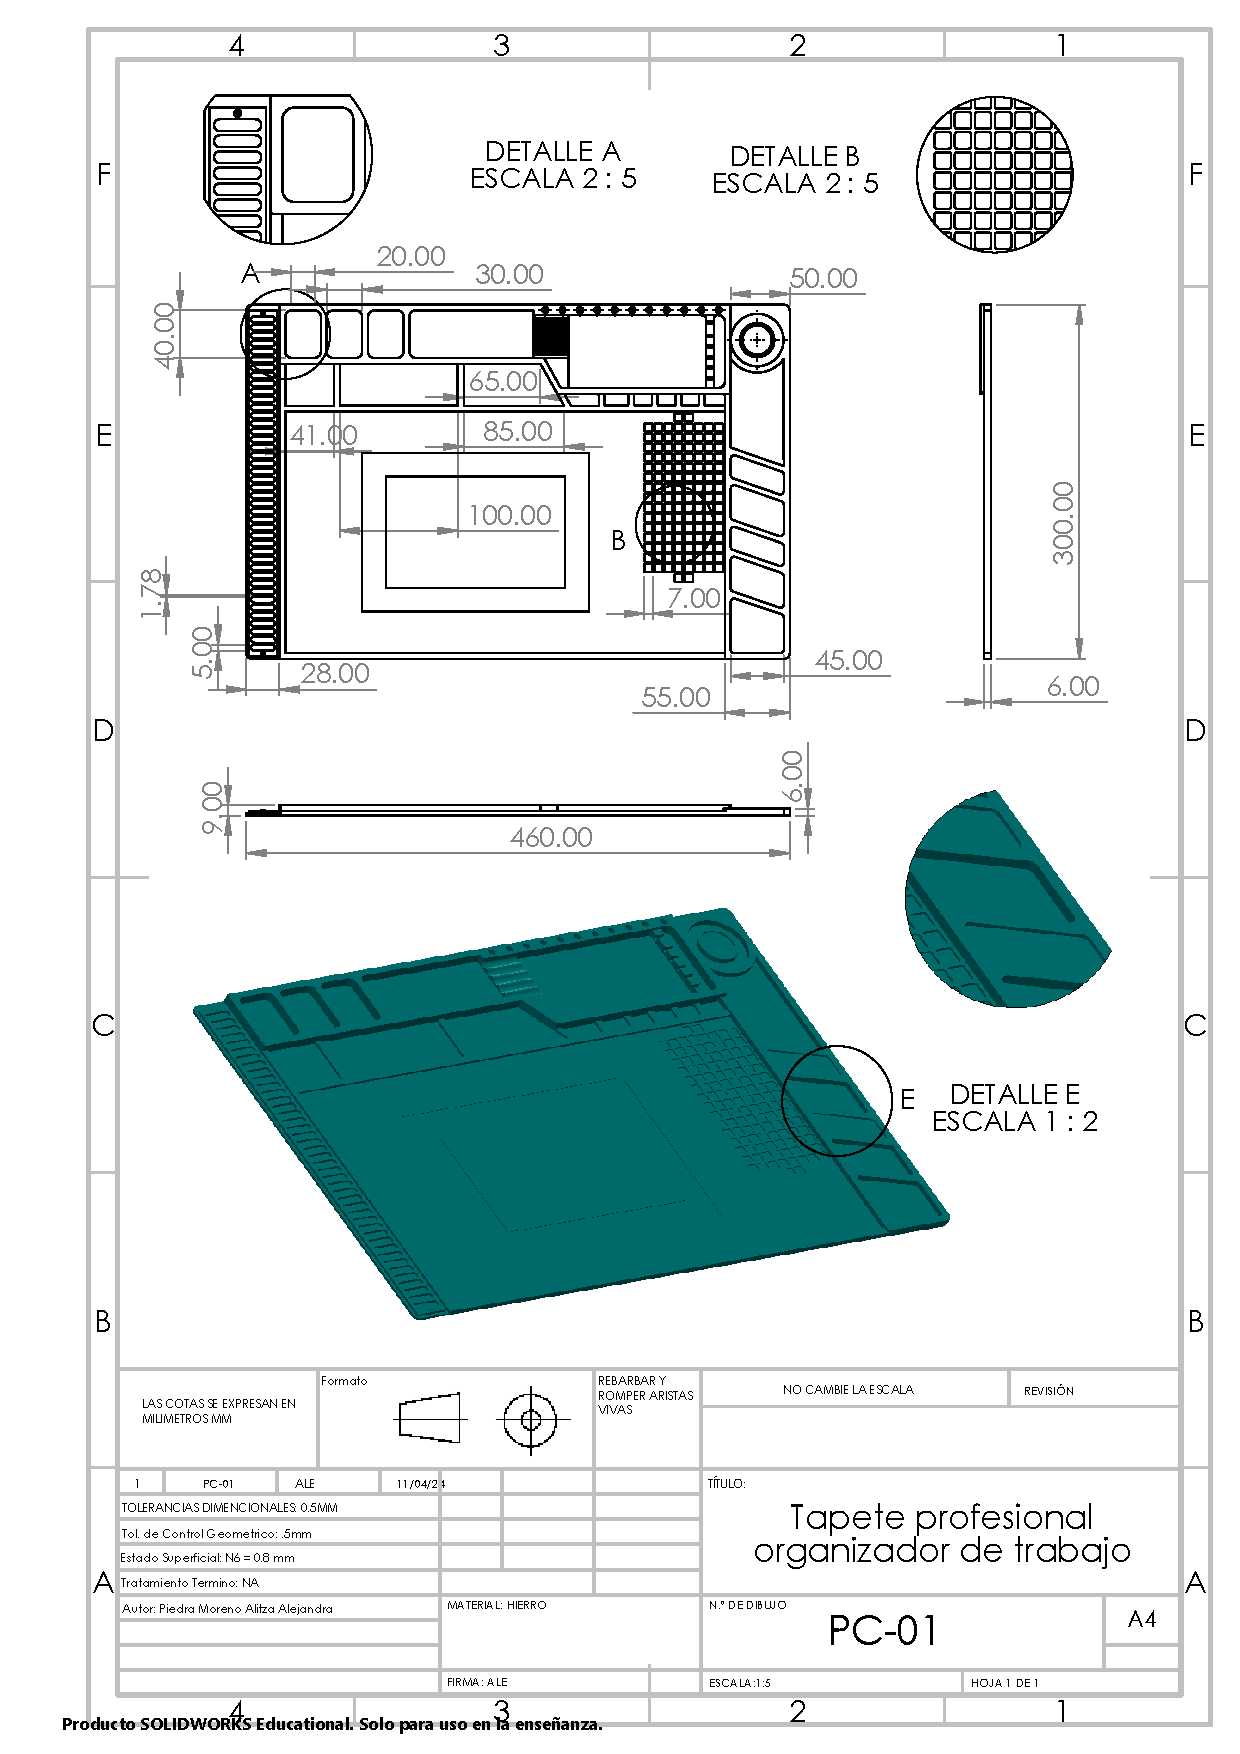
\includegraphics[trim = {7mm 1mm 1mm 1mm},clip,scale=0.4]{22/Img/almohadillaDibujo.pdf}
    \caption{Dibujo técnico de la almohadilla de trabajo}
    \label{fig:almohadillaD}
\end{figure}

Ahora que ya conocemos un poco más de la forma física de nuestro elemento, nos seguiremos a describirlo un poco más en sus propiedades, esto a razón de lo antes mencionado que es familiarizarnos primeramente con el método actual.

Propiedad antiestática: Tiene áreas especiales para colocar procesadores, microchips, memorias, tarjetas de desarrollo o cualquier otro elemento de electrónica que pueda ser afectado por la estática. Incluso, te protege de las cargas estáticas almacenadas en los componentes en reposo.


Propiedad magnética: Incorpora imanes distribuidos en lugares diferentes; perfectos para retener piezas metálicas, como tornillería, herramientas, puntas de desarmador, tarrajas y pinzas, entre otras. Además, pueden ser utilizados para magnetizar o desmagnetizar puntas de desarmadores.


Espacios ideales para el trabajo:

Minirranuras: Perfectas para colocar las piezas de los equipos desarmados y llevar el control de su posición, gracias a que están numeradas.
Minicajones: Ayudan a identificar piezas pequeñas o tornillos indispensables para el reensamblaje de los equipos en reparación.
Orificios: Útiles para que coloques tus desarmadores, aplicadores de flux o pastas en jeringa en una posición adecuada y puedas tomarlos rápidamente.
Cajones multifunción: Estos compartimentos de diversos tamaños son apropiados para otros objetos misceláneos que utilices.
Cajones con tapa: Adecuados para que almacenes y cuides los componentes más importantes.
Cajones para herramientas: Tienen el espacio ideal para colocar pinzas, espátulas, punzones y más.
Regleta: Es de 36 cm. Te servirá como referencia para trabajos en los que requieras medir.
Espacio central: Es el área de trabajo perfecta donde puedes armar o desarmar los equipos.

Material ideal para trabajar: Es flexible y tiene superficie antiderrapante. Está fabricado con silicona de textura suave al tacto que te da comodidad de uso y protege los equipos contra rayones y golpes. También puede ser usado para trabajos de soldadura, ya que soporta hasta 400 °C.



\subsubsection{PC-02: Protoboard de 300 puntos}

Un protoboard de 300 puntos es una placa de pruebas electrónica que se utiliza para prototipar circuitos electrónicos de manera temporal. Está diseñada con un patrón de agujeros y conexiones internas que permiten insertar y conectar componentes electrónicos de forma rápida y sin necesidad de soldadura. El “300 puntos” se refiere a la cantidad de puntos de conexión disponibles en la placa, lo que determina cuántos componentes y conexiones pueden alojarse en ella. Estos protoboards son herramientas muy útiles para diseñadores y estudiantes de electrónica, ya que les permiten experimentar y probar circuitos antes de realizar una implementación permanente.

En la figura \ref{fig:proto} se muestra el diseño un tanto detallado de este elemento, como podemos ver tiene una dimensión de 55 x 82 mm, estas medidas son fundamentales a la hora de realizar nuestra distribución por lo cual necesario tenerlo en cuenta además que al tener presente que es de 300 puntos podemos destinar la posición de cada una de nuestras piezas así como optimizar nuestro ensamble.

\begin{figure}[H]
    \centering
    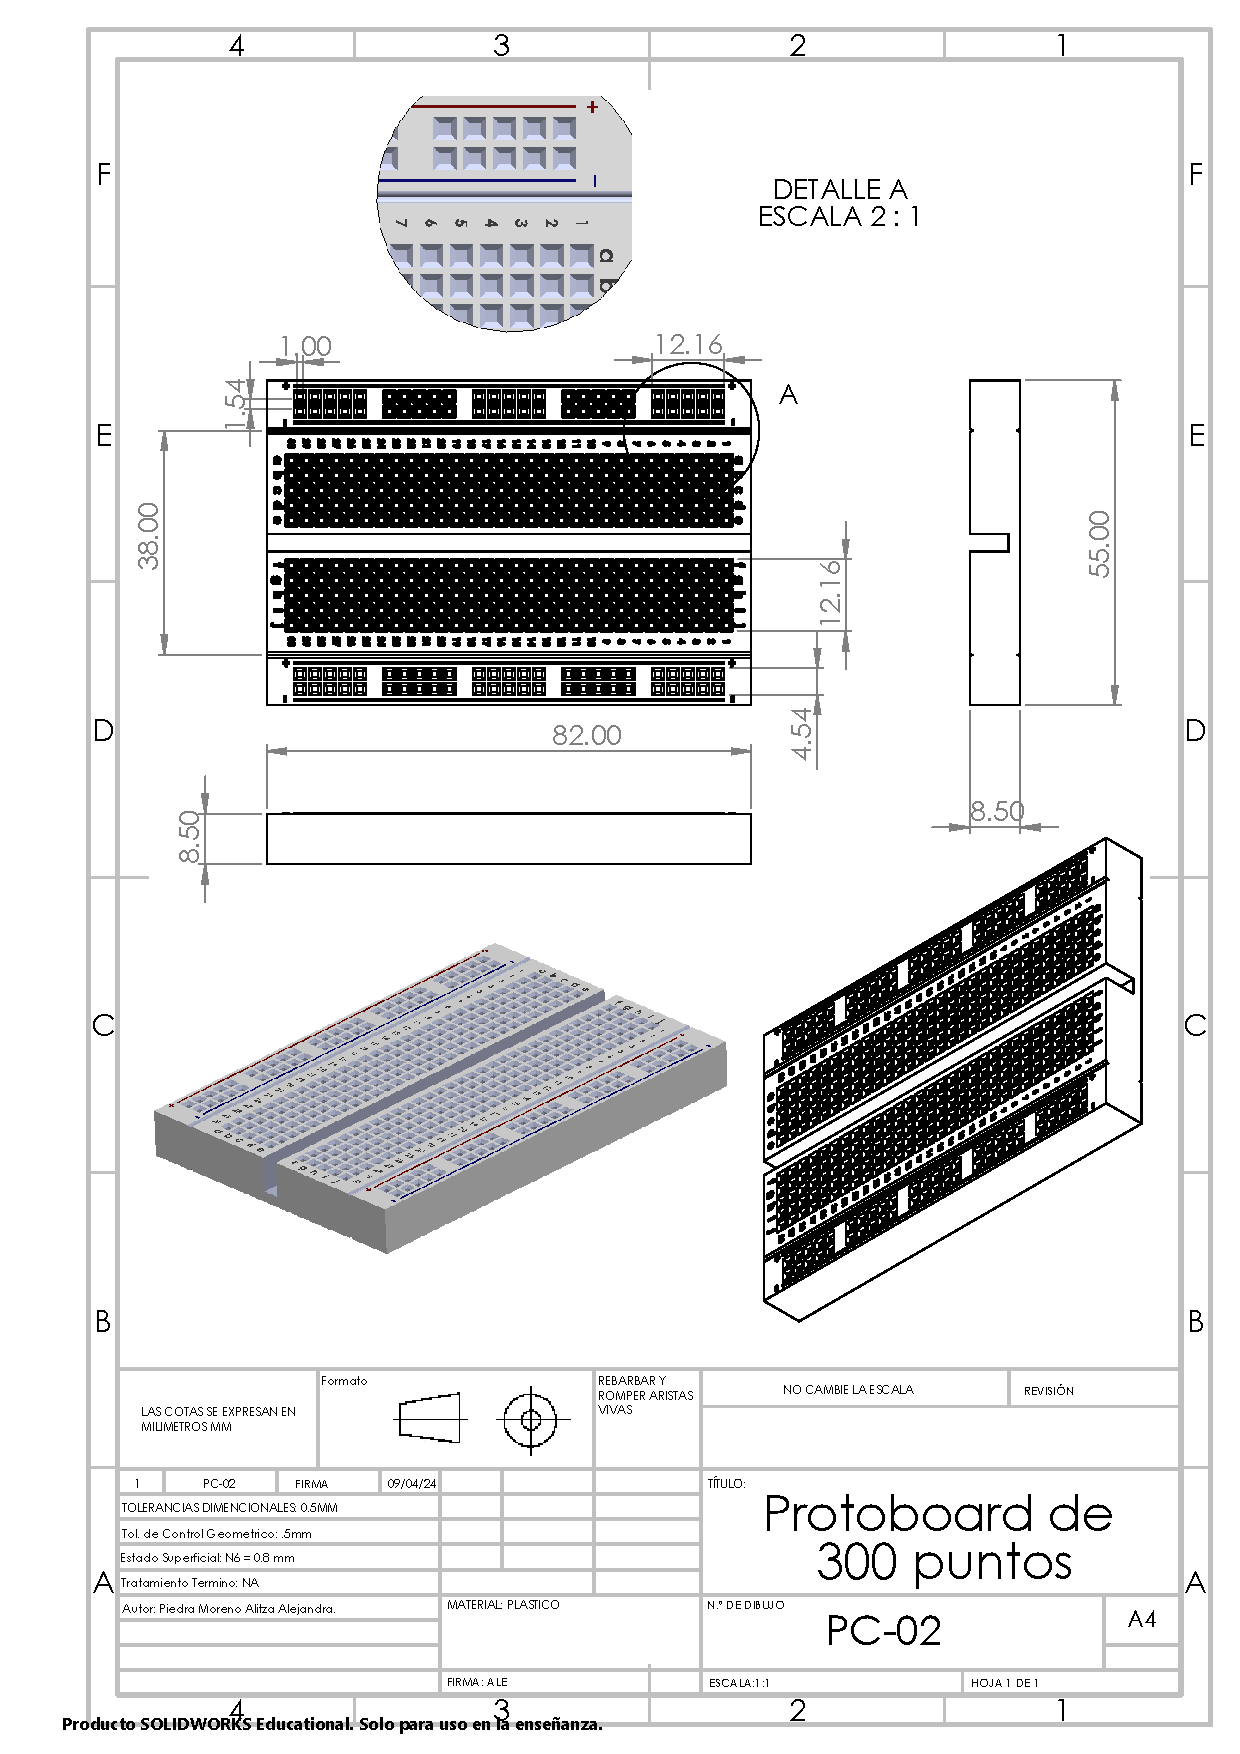
\includegraphics[trim = {7mm 1mm 1mm 1mm},clip,scale=0.4]{22/Img/protoDibujo.pdf}
    \caption{Dibujo técnico del protoboard de 300 puntos}
    \label{fig:proto}
\end{figure}

\subsubsection{PC-03: Pantalla de cristal líquido (LCD) 16X2}

Una pantalla de cristal líquido (LCD) 16x2 es un tipo común de pantalla de visualización utilizada en una variedad de dispositivos electrónicos, como relojes, calculadoras, equipos de prueba, sistemas de control, y muchos otros dispositivos electrónicos. La designación “16x2” se refiere a la cantidad de caracteres que puede mostrar la pantalla en cada línea y el número de líneas, respectivamente, el 16, indica que la pantalla tiene 16 caracteres en cada línea horizontal. Esto significa que puede mostrar hasta 16 caracteres en una fila antes de pasar a la siguiente línea, mientras que el 2 indica que la pantalla tiene 2 líneas verticales de caracteres. Por lo tanto, puede mostrar dos líneas de texto o caracteres simultáneamente.

Las pantallas LCD 16x2 generalmente funcionan con un controlador que facilita la comunicación con un microcontrolador o un dispositivo de procesamiento similar. Estas pantallas están compuestas por un conjunto de segmentos de cristal líquido que se activan eléctricamente para mostrar caracteres alfanuméricos, símbolos y otros tipos de información visual. Las pantallas LCD son populares debido a su bajo consumo de energía y su capacidad para mostrar información de manera clara y legible en una variedad de condiciones de iluminación.

En la figura \ref{fig:lcd} se muestra el dibujo técnico de esta pantalla LCD, donde nos muestra dimensiones importantes que se deben tener en cuenta en nuestro análisis. Como se observa, la placa base de la lcd tiene una dimensión de 80x36 mm, además que podemos observar que contiene 16 pines o patitas que son las que nos permite mandarle señales a nuestra pantalla y a través de la interfaz esta tarea se nos facilita muchísimo más.

\begin{figure}[H]
    \centering
    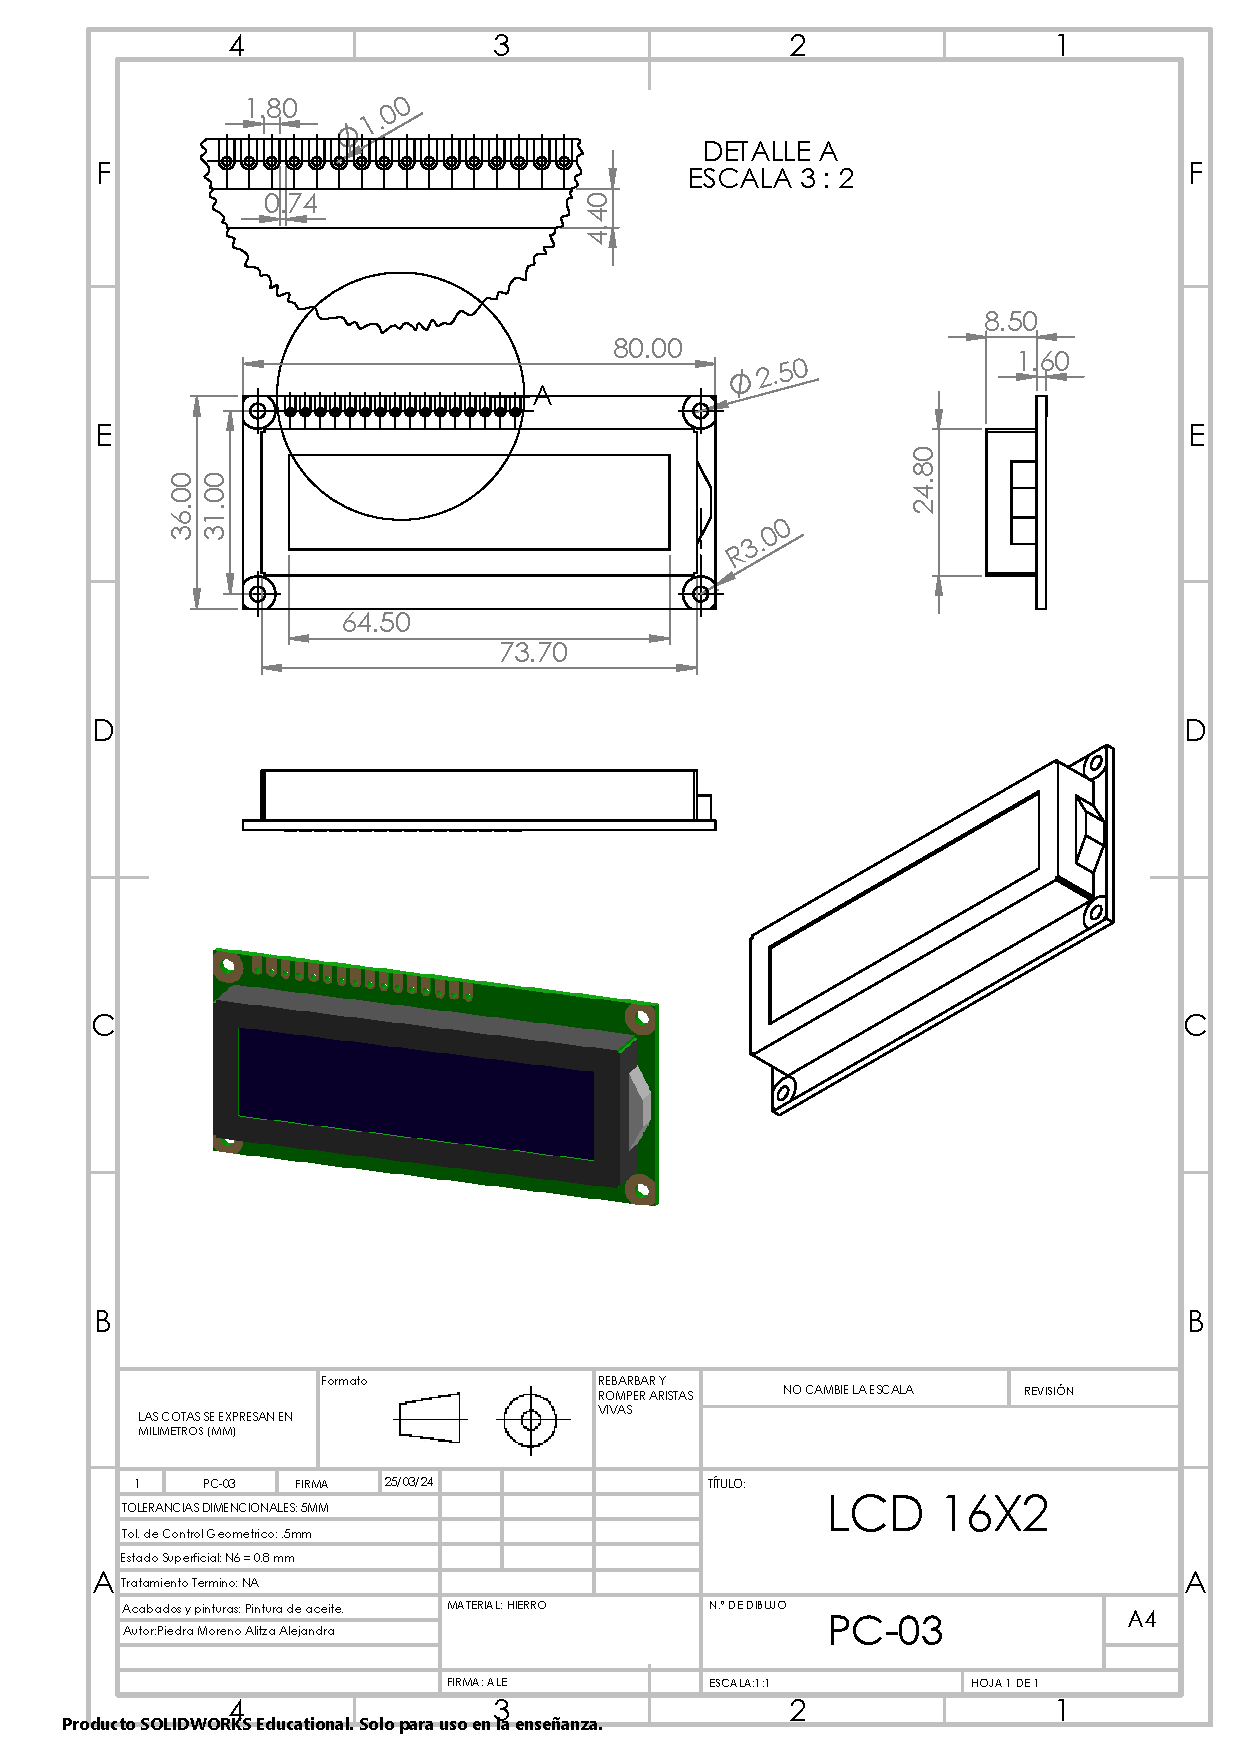
\includegraphics[trim = {7mm 1mm 1mm 1mm},clip,scale=0.4]{22/Img/lcdDibujo.PDF}
    \caption{Dibujo técnico de una LCD 16X2}
    \label{fig:lcd}
\end{figure}

\subsubsection{PC-04: Módulo I2C Interfaz LCD 16x2 }

El módulo I2C Interfaz LCD 16x2 es un dispositivo que combina una pantalla LCD alfanumérica de 16 caracteres por 2 líneas con un controlador integrado y una interfaz de comunicación I2C. Este tipo de módulos se utilizan comúnmente en proyectos de electrónica y sistemas embebidos para proporcionar una interfaz de usuario visual.

El funcionamiento del módulo I2C Interfaz LCD 16x2 es relativamente simple:

Conexión física: El módulo se conecta a un microcontrolador u otro dispositivo maestro a través de dos cables: uno para la línea de datos (SDA) y otro para la línea de reloj (SCL) del bus I2C. Estas conexiones permiten que el microcontrolador envíe comandos y datos al módulo LCD.

Inicialización: Antes de poder utilizar la pantalla LCD, es necesario inicializarla. Esto implica configurar el controlador del LCD para que se comunique correctamente con el microcontrolador y establecer parámetros como el contraste, el brillo y la posición del cursor.

Envío de datos: Una vez inicializado, el microcontrolador puede enviar comandos y datos al módulo LCD a través del bus I2C. Estos datos pueden incluir caracteres individuales para mostrar en la pantalla, comandos de control para configurar el comportamiento del LCD (como borrar la pantalla, mover el cursor, etc.), o incluso mensajes completos que deben mostrarse en la pantalla.

Actualización de la pantalla: El controlador del módulo LCD se encarga de traducir los comandos y datos recibidos del microcontrolador en acciones específicas en la pantalla. Esto puede incluir la activación y desactivación de píxeles individuales para mostrar caracteres, la actualización de la posición del cursor en la pantalla, o cualquier otra operación necesaria para reflejar los datos enviados por el microcontrolador en la pantalla LCD.

En la siguiente figura \ref{fig:modulo} se muestran las medidas y detalles importantes que se deben conocer de este módulo de LCD
\begin{figure}[H]
    \centering
    \includegraphics[trim = {7mm 1mm 1mm 1mm},clip,scale=0.4]{22/Img/móduloI2CInterfazDibujo.pdf}
    \caption{Dibujo técnico: Módulo I2C Interfaz LCD 16x2}
    \label{fig:modulo}
\end{figure}


\subsubsection{PC-05: ESP32-C6-WROOM-1 }

El ESP32-C6-WROOM-1 es un módulo de conectividad WiFi y Bluetooth fabricado por Espressif Systems. Forma parte de la familia de microcontroladores ESP32, que son muy populares en el mundo de la electrónica y la Internet de las cosas (IoT) debido a su potencia, versatilidad y bajo costo.

Aquí hay algunas características clave del ESP32-C6-WROOM-1:

1. Conectividad WiFi: El módulo ofrece conectividad WiFi de doble banda (2.4 GHz y 5 GHz), lo que permite la comunicación inalámbrica con redes locales y acceso a Internet.

2. Conectividad Bluetooth: Además del WiFi, el ESP32-C6-WROOM-1 también admite Bluetooth Classic y Bluetooth de baja energía (BLE), lo que lo hace adecuado para aplicaciones que requieren interacción inalámbrica con dispositivos cercanos, como teléfonos inteligentes, sensores, etc.

3. Procesador potente: El ESP32-C6-WROOM-1 está equipado con un potente procesador de aplicación Tensilica Xtensa de 32 bits, que proporciona el poder de procesamiento necesario para ejecutar aplicaciones complejas y manejar múltiples tareas simultáneamente.

4. Memoria integrada: El módulo cuenta con una cantidad suficiente de memoria flash y RAM integrada para almacenar el firmware del sistema, datos de la aplicación y variables temporales durante la ejecución del programa.

5. Interfaces de periféricos: Ofrece una amplia gama de interfaces de periféricos, como UART, SPI, I2C, I2S, PWM, ADC, DAC, etc., que permiten la conexión con una variedad de sensores, actuadores y otros dispositivos externos.

6. Seguridad: El ESP32-C6-WROOM-1 incluye características de seguridad como Secure Boot, Flash Encryption y cifrado de datos para garantizar la integridad y confidencialidad de los datos transmitidos y almacenados.

En resumen, el ESP32-C6-WROOM-1 es un módulo altamente integrado y versátil que proporciona conectividad WiFi y Bluetooth junto con un potente procesador y una variedad de interfaces de periféricos, lo que lo hace ideal para una amplia gama de aplicaciones IoT y proyectos de electrónica.

Para que el operario se familiarice, como en las demás piezas, en la figura \ref{fig:esp} se muestra el dibujo técnico de nuestra pieza.
\begin{figure}[H]
    \centering
    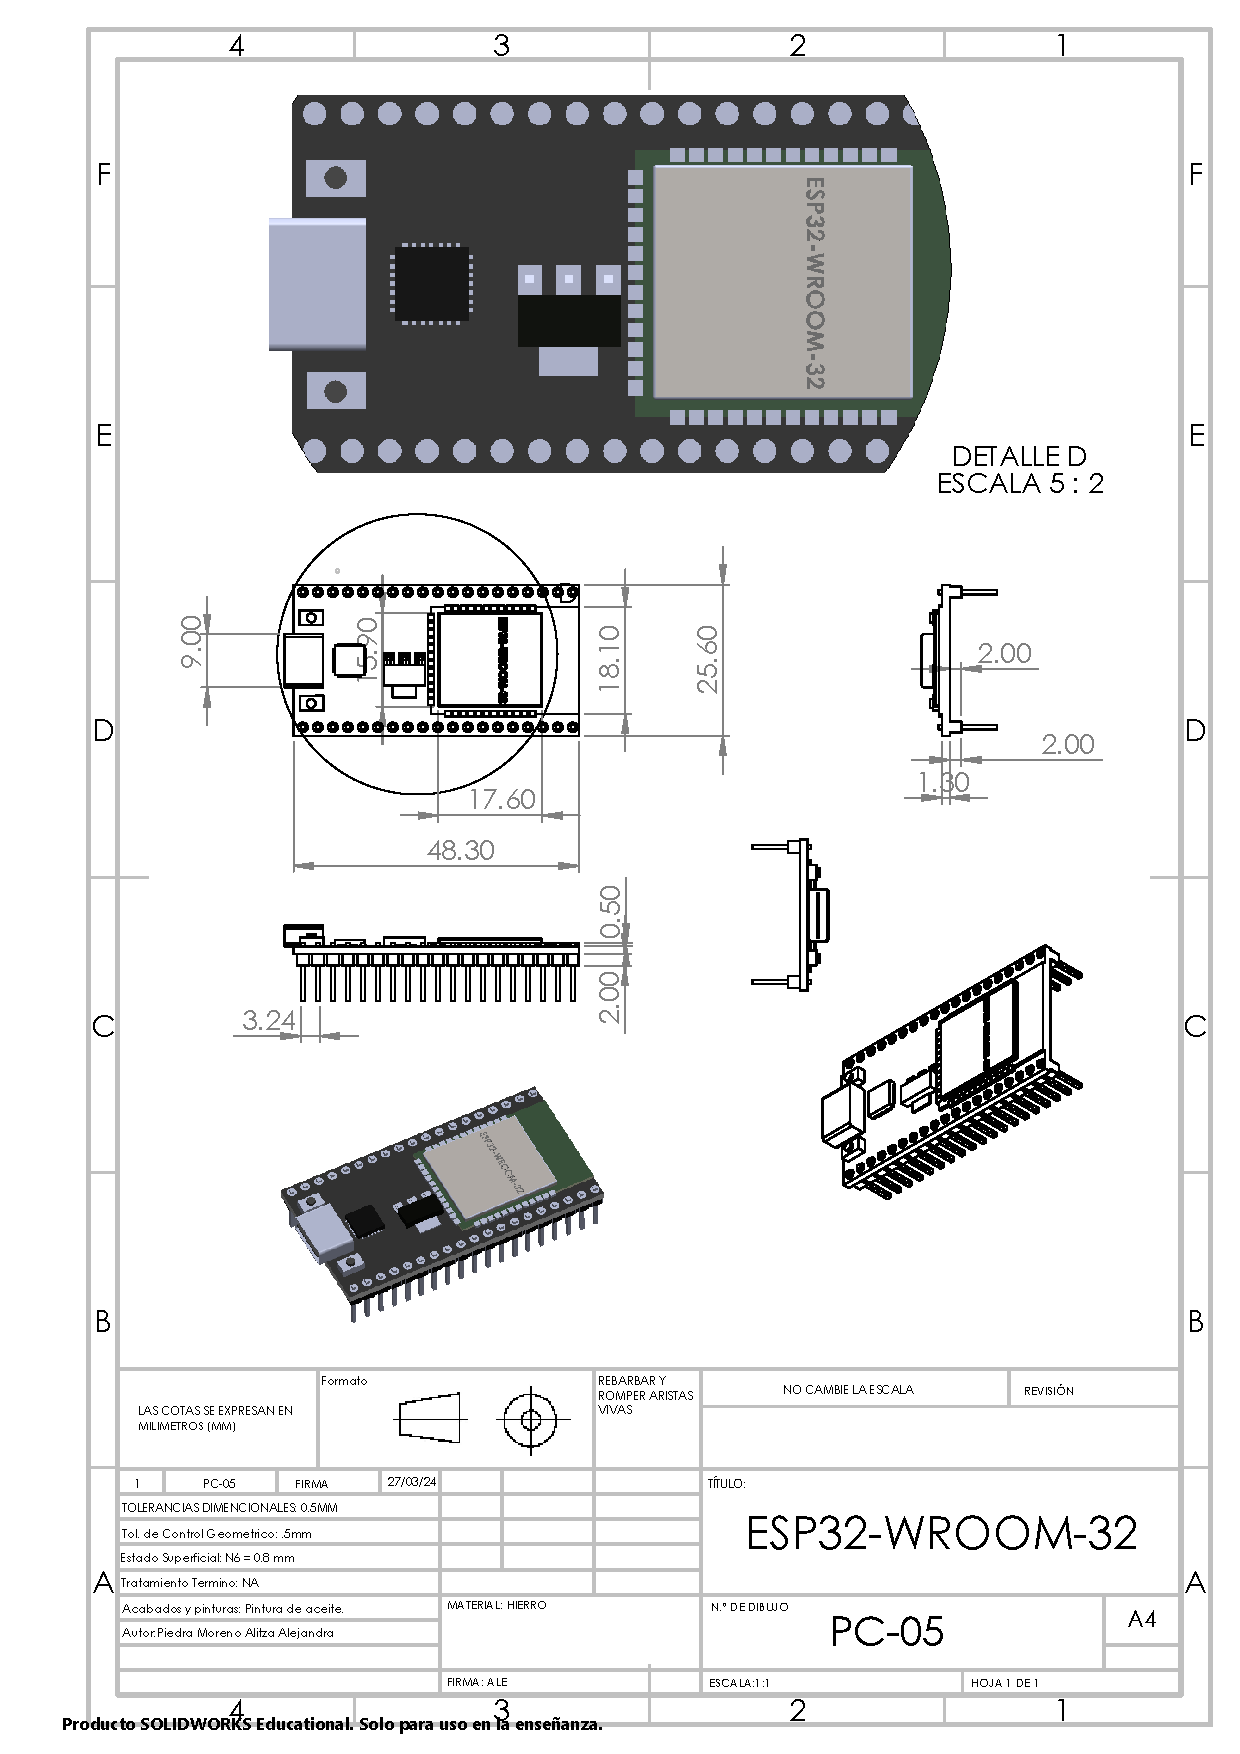
\includegraphics[trim = {7mm 1mm 1mm 1mm},clip,scale=0.4]{22/Img/esp32Dibujo.pdf}
    \caption{Dibujo técnico: ESP32-C6-WROOM-1}
    \label{fig:esp}
\end{figure}

\subsubsection{PC-06: Potenciómetro lineal 1k preciso }
Un potenciómetro es un dispositivo conformado por 2 resistencias en serie, las cuales poseen valores que pueden ser modificados por el usuario. 


\begin{figure}[H]
    \centering
    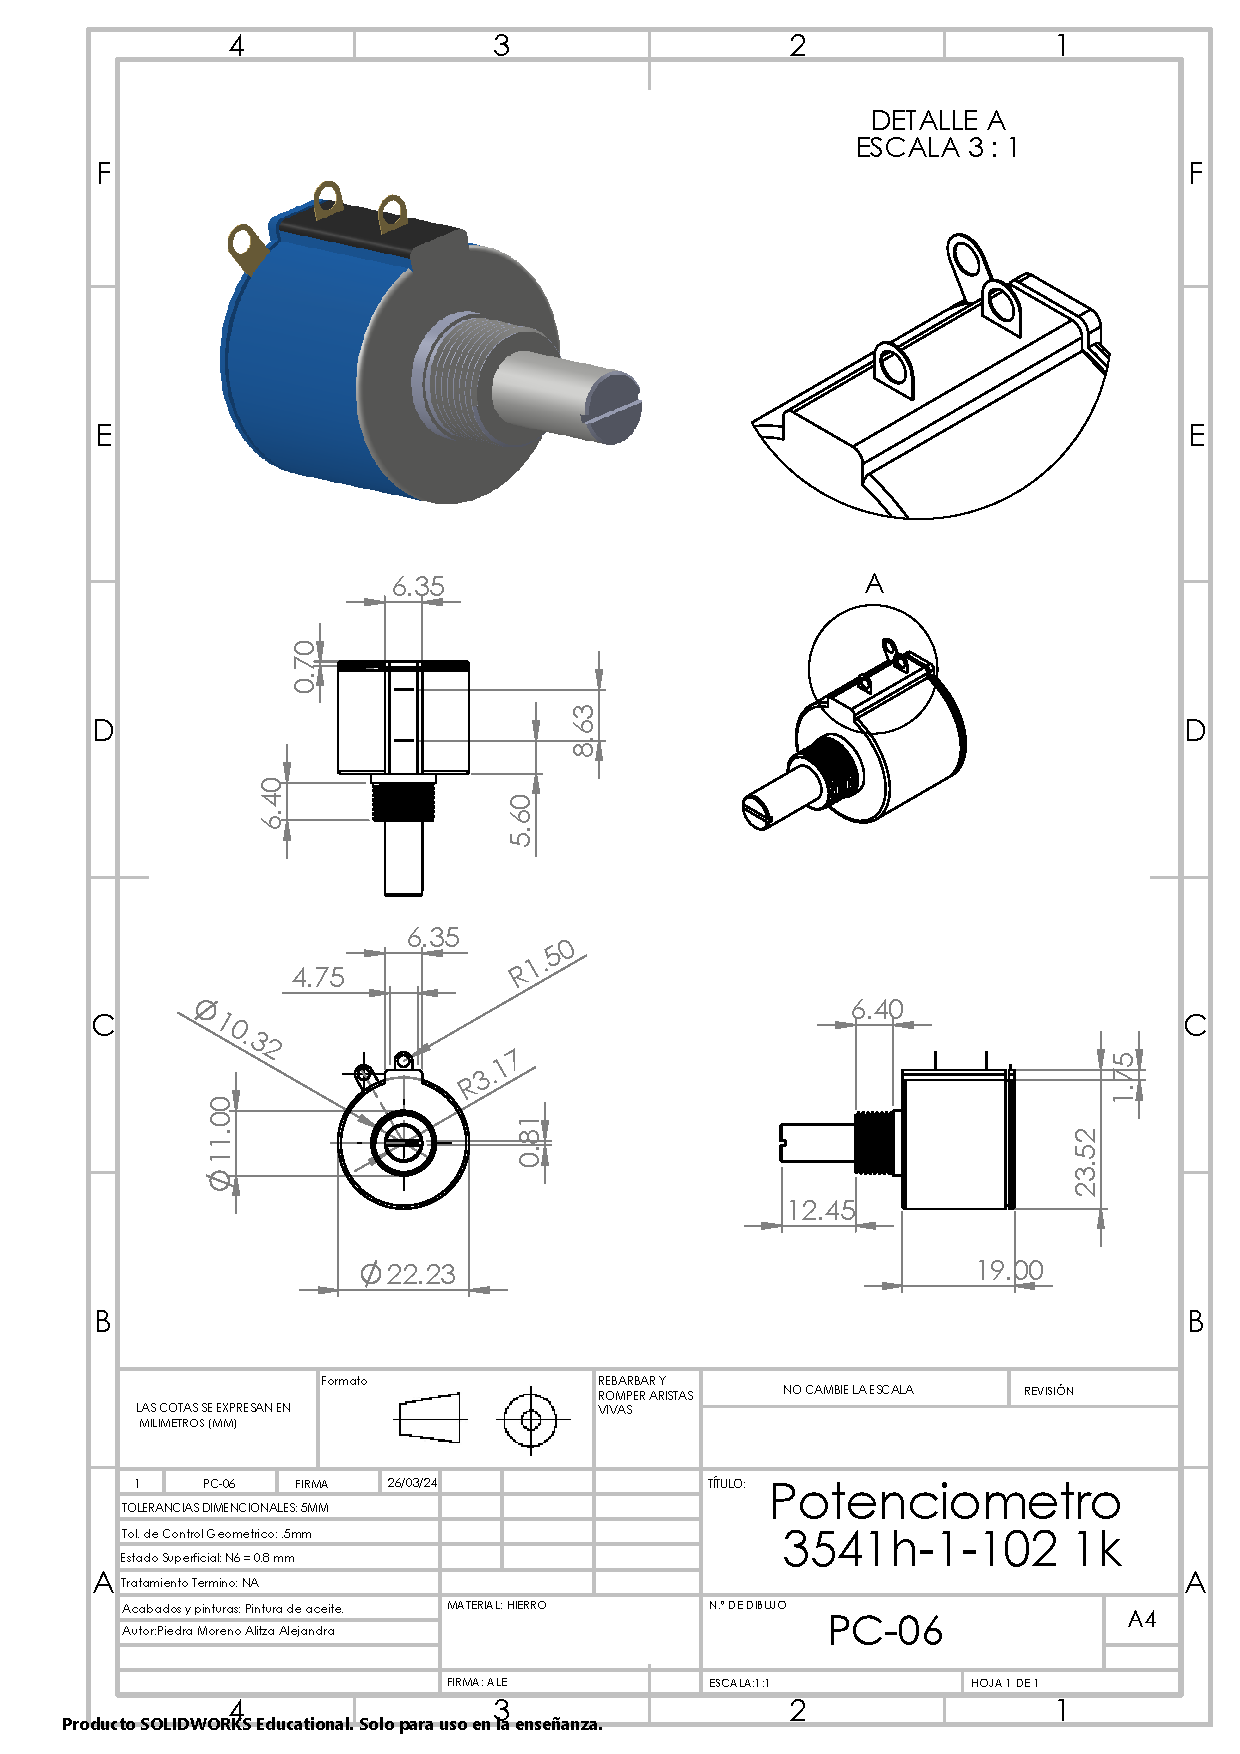
\includegraphics[trim = {7mm 1mm 1mm 1mm},clip,scale=0.4]{22/Img/potenciometroDibujo.PDF}
    \caption{Dibujo técnico: Potenciómetro lineal 1k preciso}
    \label{fig:potenciometro}
\end{figure}


\subsubsection{PC-07: Resistencia de 330 ohms 1/4 W }
La resistencia es una medida de la oposición al flujo de corriente en un circuito eléctrico.

La resistencia se mide en ohmios, que se simbolizan con la letra griega omega ($\Omega$). Se denominaron ohmios en honor a Georg Simon Ohm (1784-1854), un físico alemán que estudió la relación entre voltaje, corriente y resistencia. Se le atribuye la formulación de la ley de Ohm.

Todos los materiales resisten en cierta medida el flujo de corriente. Se incluyen en una de dos amplias categorías:

Conductores: materiales que ofrecen muy poca resistencia, donde los electrones pueden moverse fácilmente. Ejemplos: plata, cobre, oro y aluminio.
Aislantes: materiales que presentan alta resistencia y restringen el flujo de electrones. Ejemplos: goma, papel, vidrio, madera y plástico.
Normalmente, se toman las mediciones de resistencia para indicar las características de un componente o un circuito.

Cuanto mayor sea la resistencia, menor será el flujo de corriente. Si es anormalmente alta, una causa posible (entre muchas) podrían ser los conductores dañados por el fuego o la corrosión. Todos los conductores emiten cierto grado de calor, por lo que el sobrecalentamiento es un problema que a menudo se asocia con la resistencia.

Cuanto menor sea la resistencia, mayor será el flujo de corriente. Causas posibles: aisladores dañados por la humedad o un sobrecalentamiento.
Muchos componentes, tales como los elementos de calefacción y las resistencias, tienen un valor de resistencia fijo. Estos valores se imprimen a menudo en las placas de identificación de los componentes o en los manuales de referencia.

Cuando se indica una tolerancia, el valor de resistencia debe encontrarse dentro de la gama de la resistencia especificada. Cualquier cambio significativo en un valor de resistencia fijo generalmente indica un problema.
 %https://www.fluke.com/es-mx/informacion/blog/electrica/que-es-la-resistencia%
 
\begin{figure}[H]
    \centering
    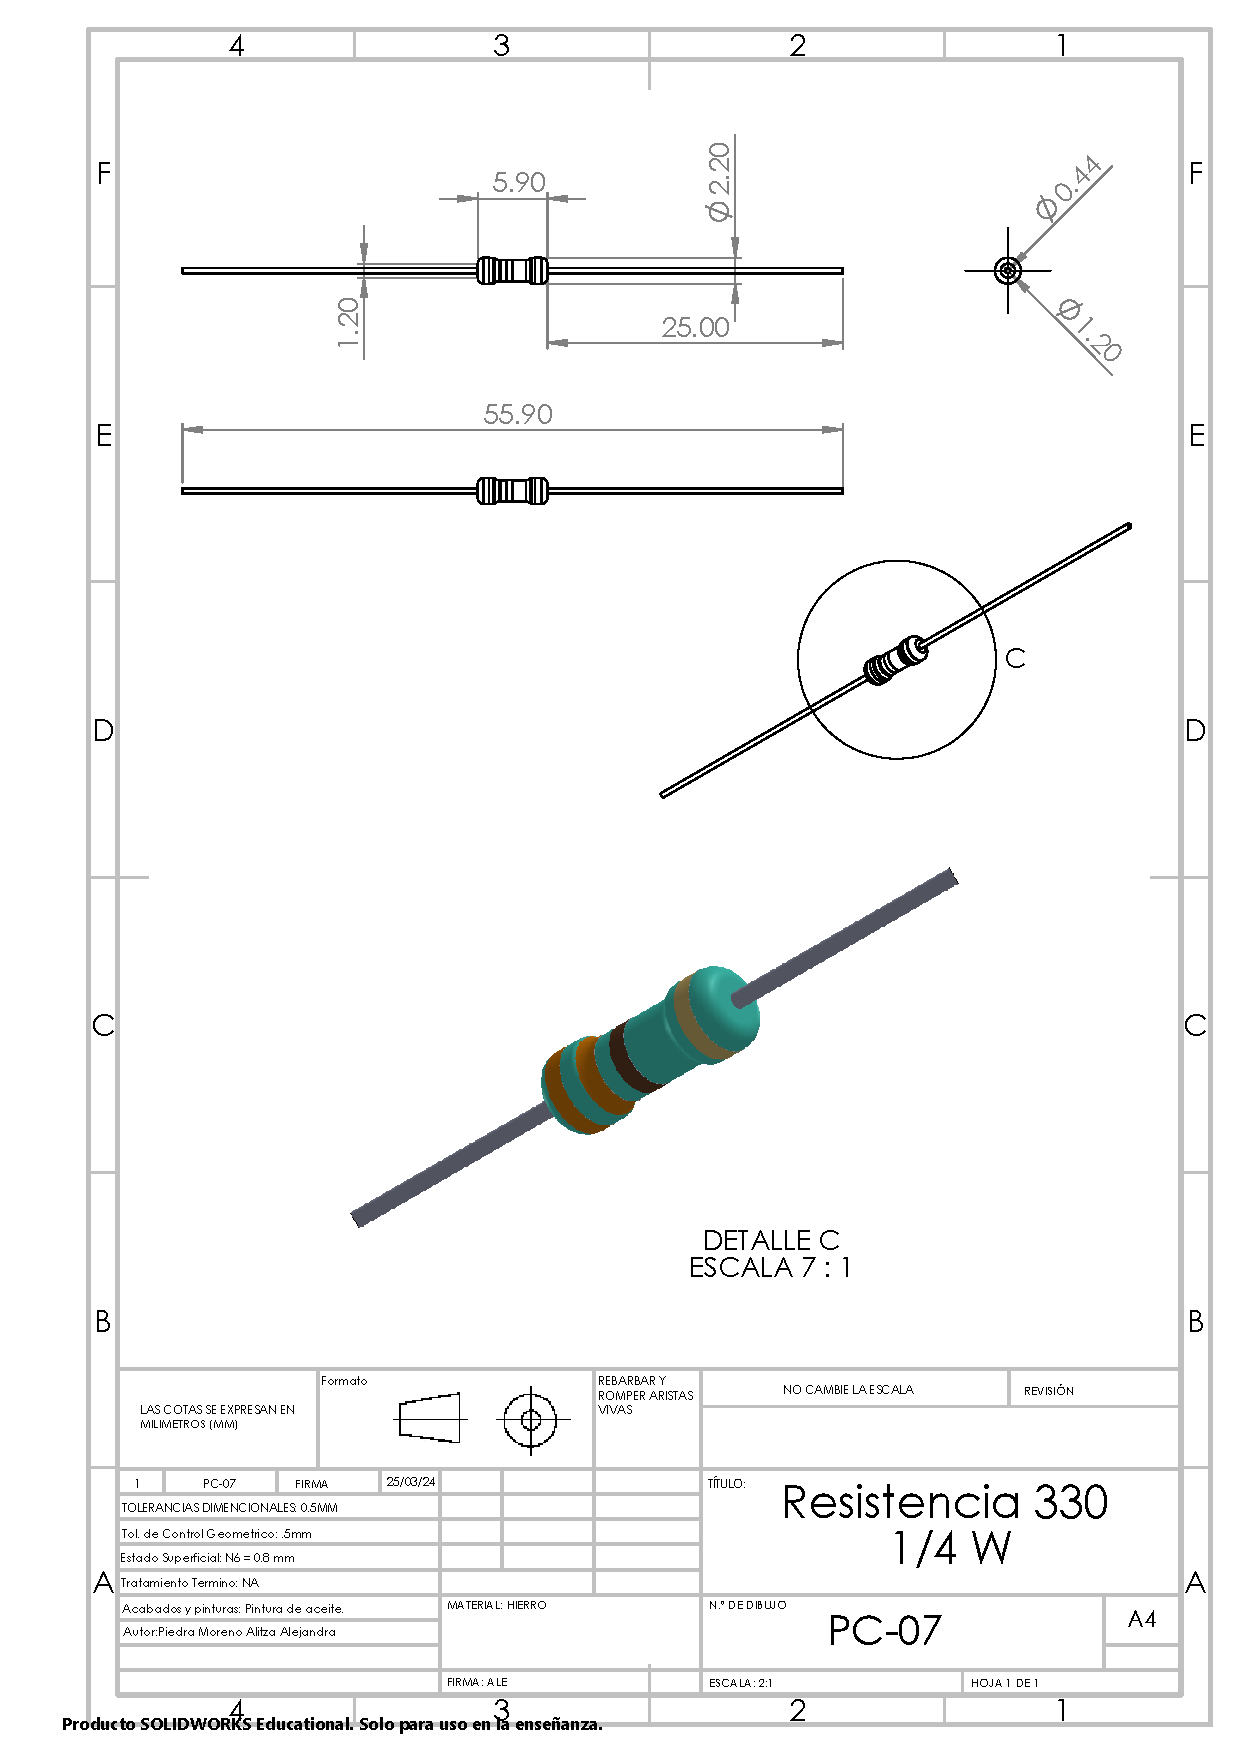
\includegraphics[trim = {7mm 1mm 1mm 1mm},clip,scale=0.4]{22/Img/resistenciaDibujo.PDF}
    \caption{Dibujo técnico: Resistencia de 330 ohms 1/4 W}
    \label{fig:enter-label7}
\end{figure}


\subsubsection{PC-08: Cables Dupont }

Se utilizan principalmente como cables puente en protoboards y para interconectar tarjetas de desarrollo con sensores, módulos, actuadores, motores, etc. Suelen verse mucho en proyectos con Arduino o Raspberry Pi y son un material que se ha vuelto indispensable para estudiantes que trabajan con circuitos electrónicos. 

\begin{figure}[H]
    \centering
    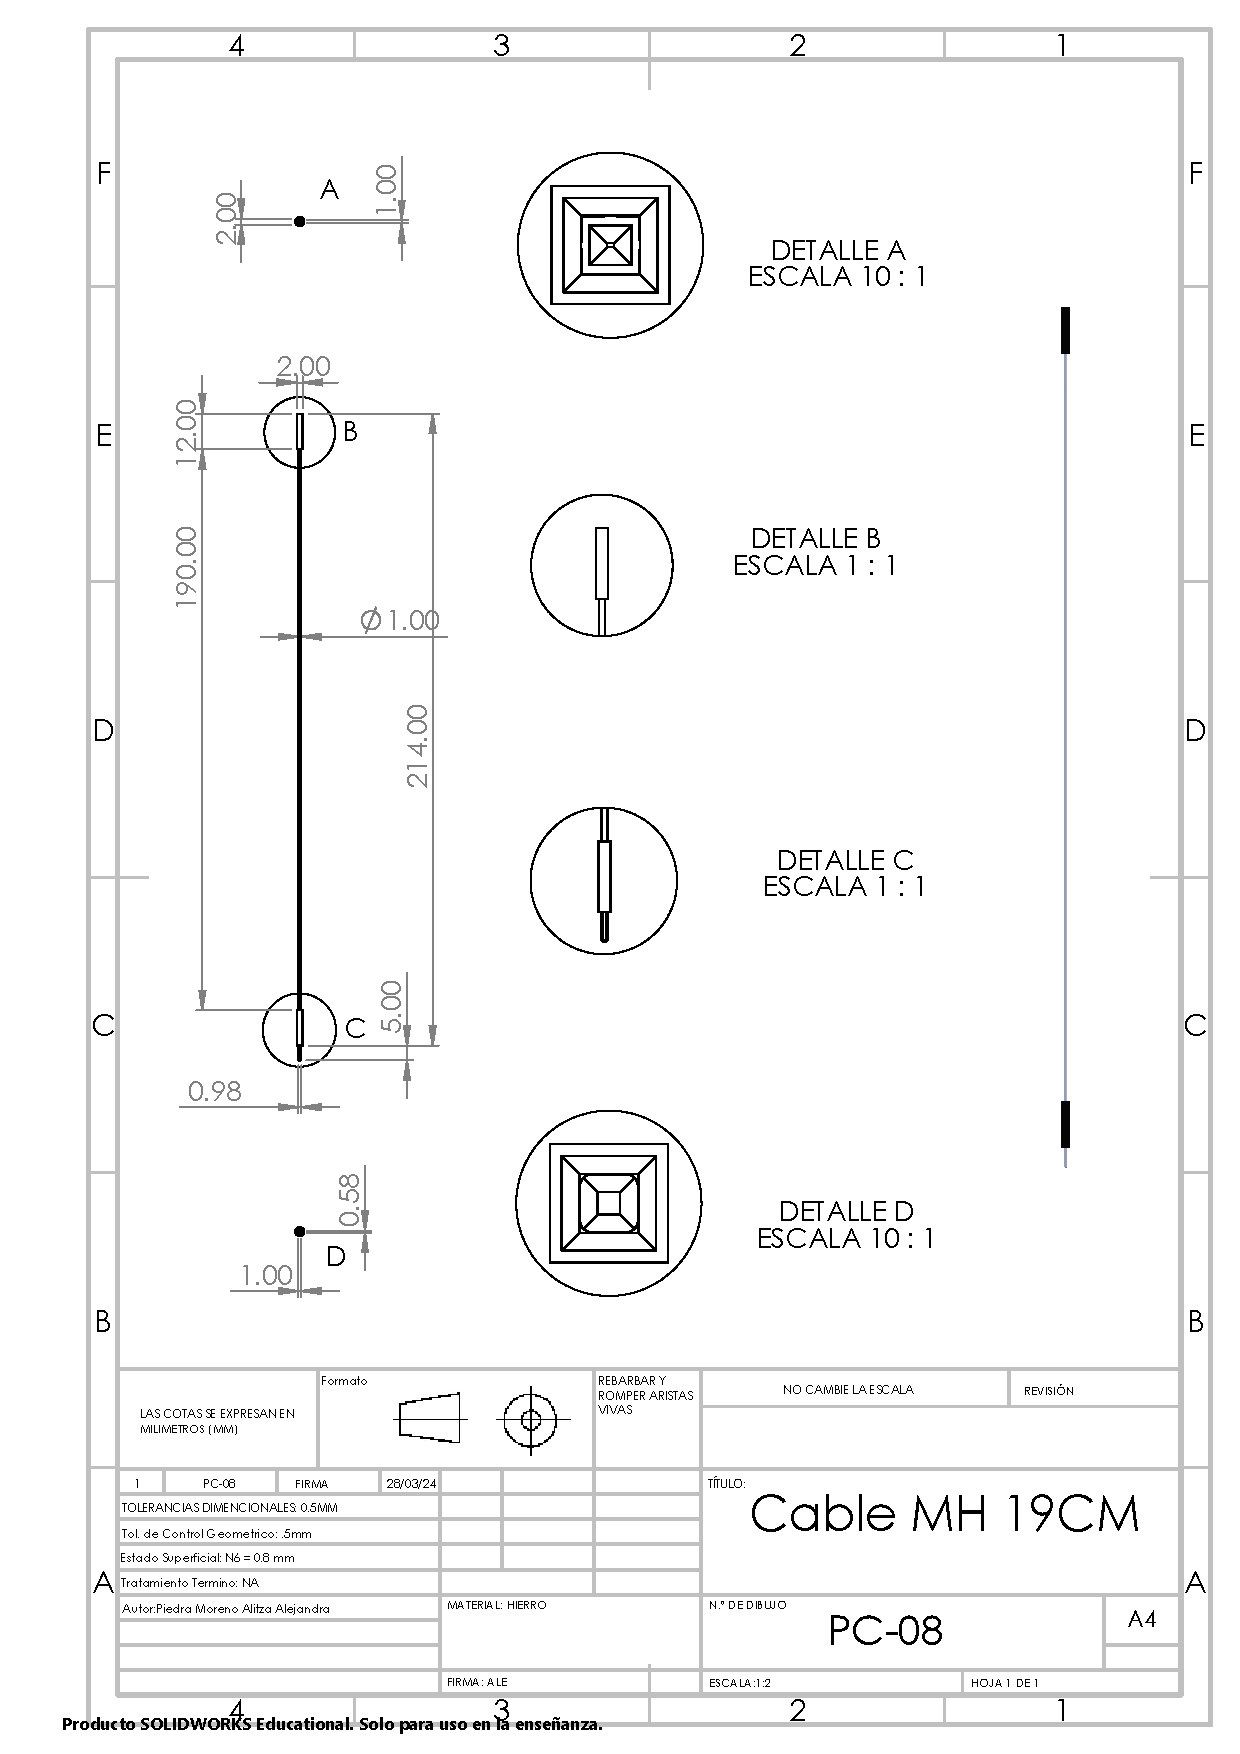
\includegraphics[trim = {7mm 1mm 1mm 1mm},clip,scale=0.4]{22/Img/cableMHDibujo.PDF}
    \caption{Dibujo técnico: Cable MH}
    \label{fig:enter-label8}
\end{figure}

\begin{figure}[H]
    \centering
    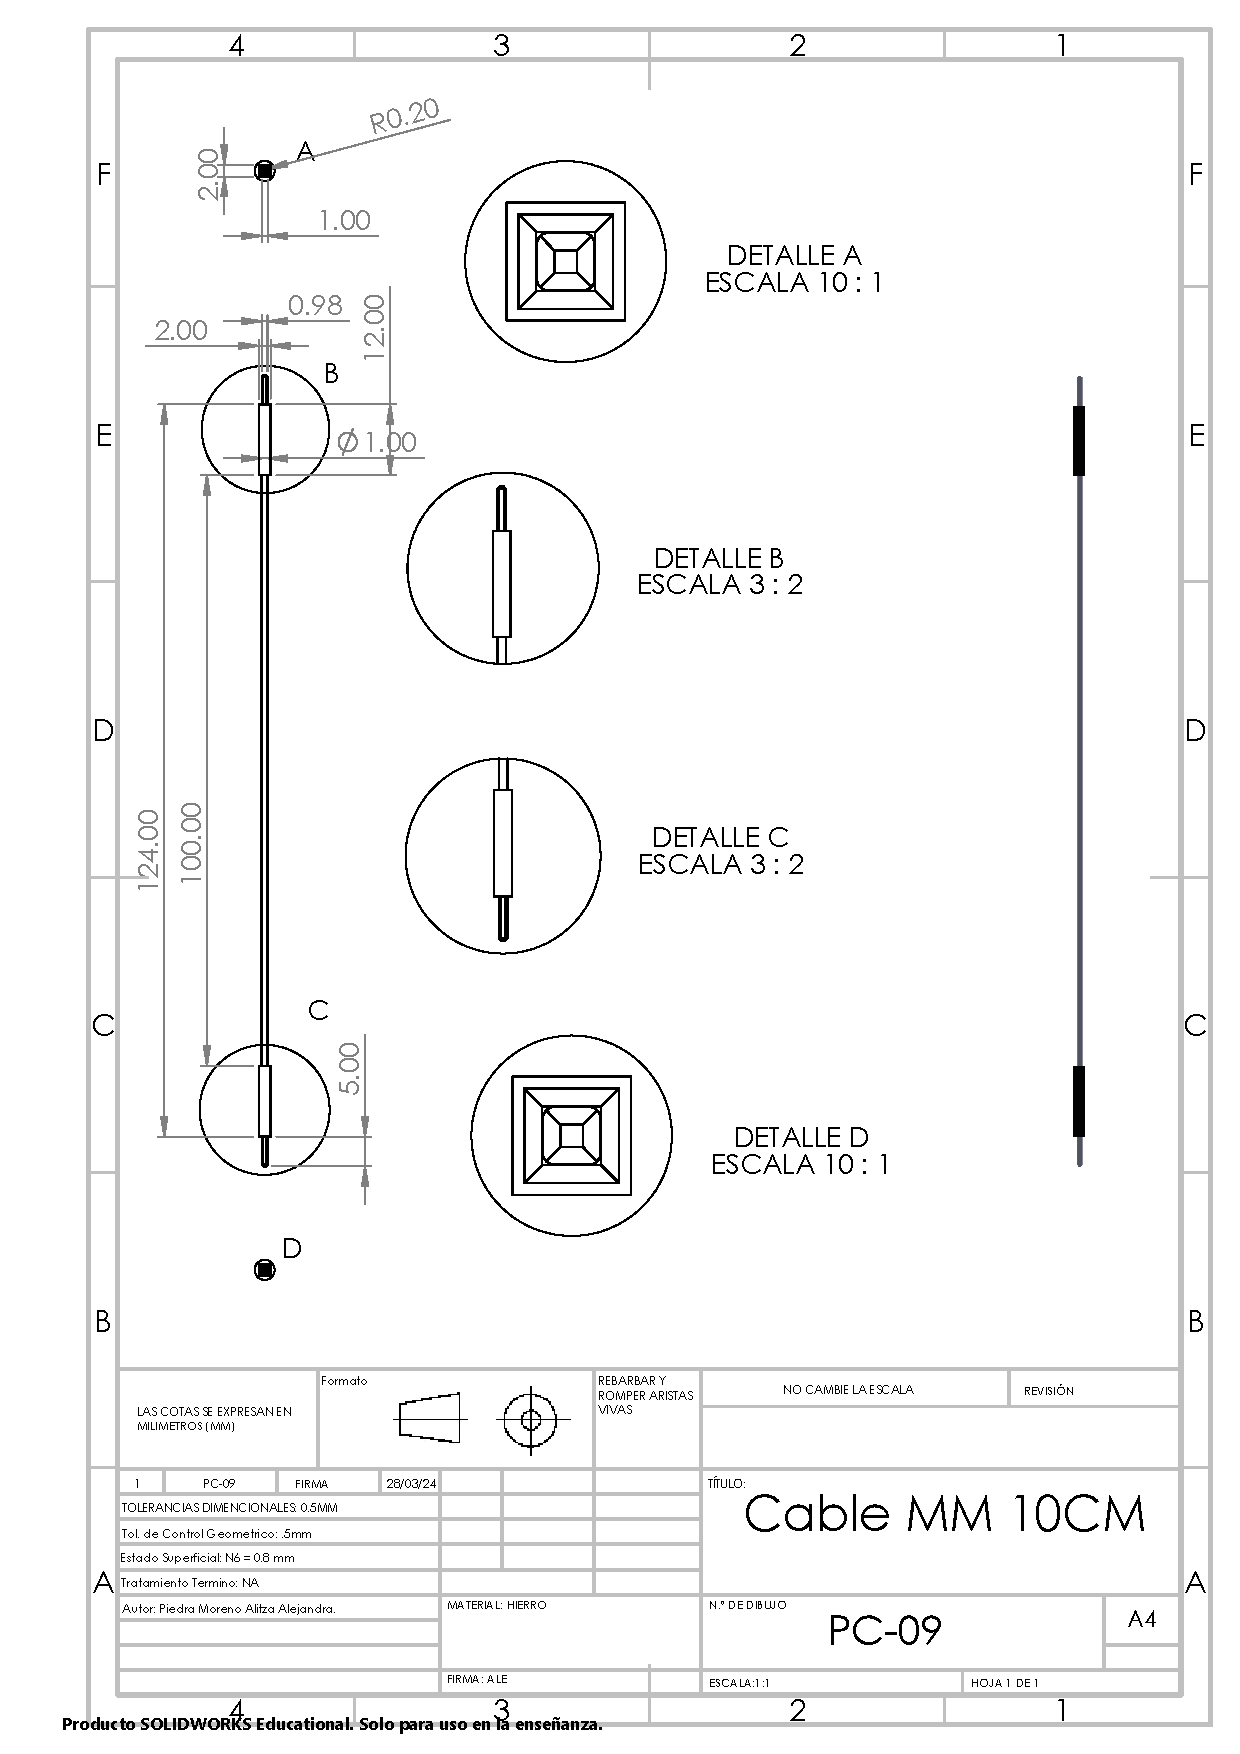
\includegraphics[trim = {7mm 1mm 1mm 1mm},clip,scale=0.4]{22/Img/cableMMDibujo.PDF}
    \caption{Dibujo técnico: Cable MM}
    \label{fig:enter-label9}
\end{figure}

\subsubsection{PC-10: Regulador Multicontacto Con 8 Salidas 3 Usb Y 1 Tipo C }
\begin{figure}[H]
    \centering
    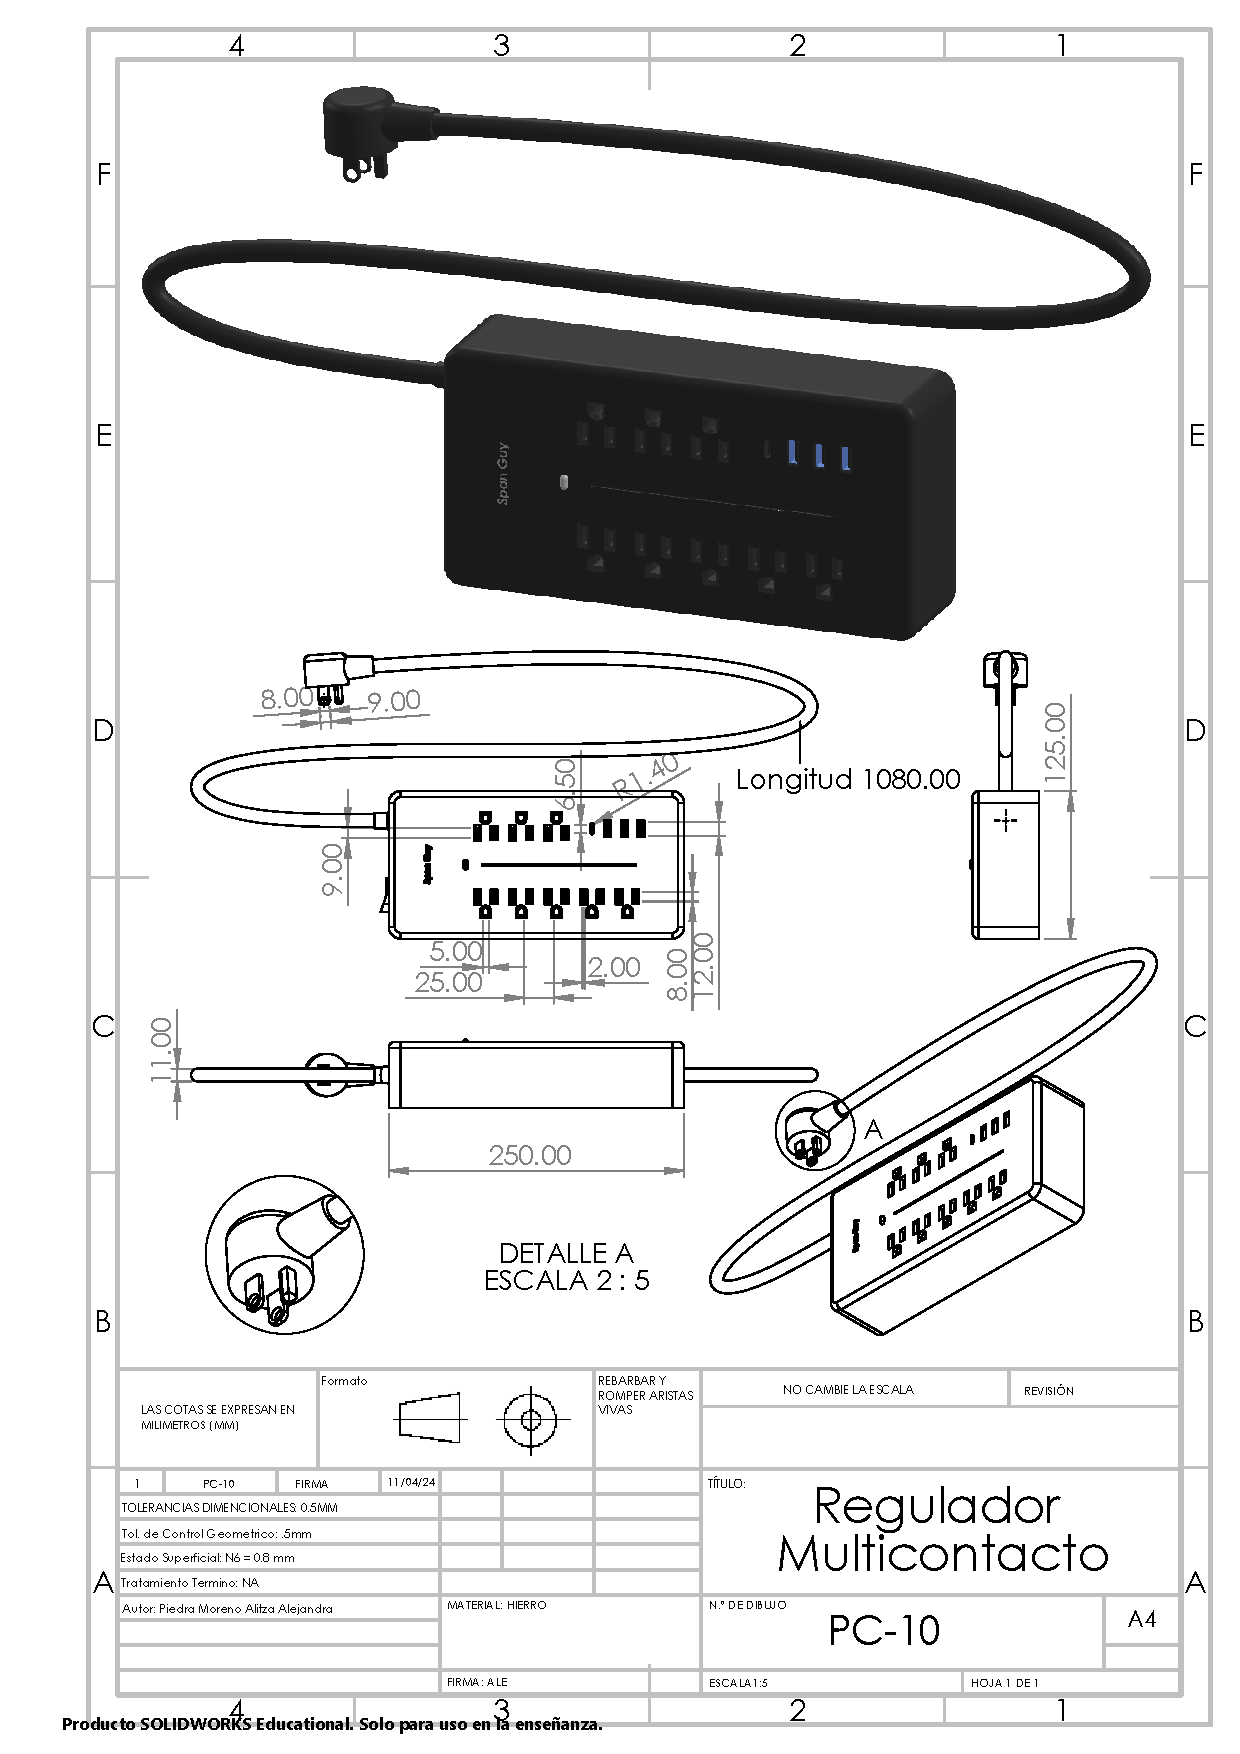
\includegraphics[trim = {7mm 1mm 1mm 1mm},clip,scale=0.4]{22/Img/multicontactoDibujo.pdf}
    \caption{Dibujo técnico: Cable MM}
    \label{fig:enter-label9}
\end{figure}

\subsubsection{PC-11: Cable Tipo C }
\begin{figure}[H]
    \centering
    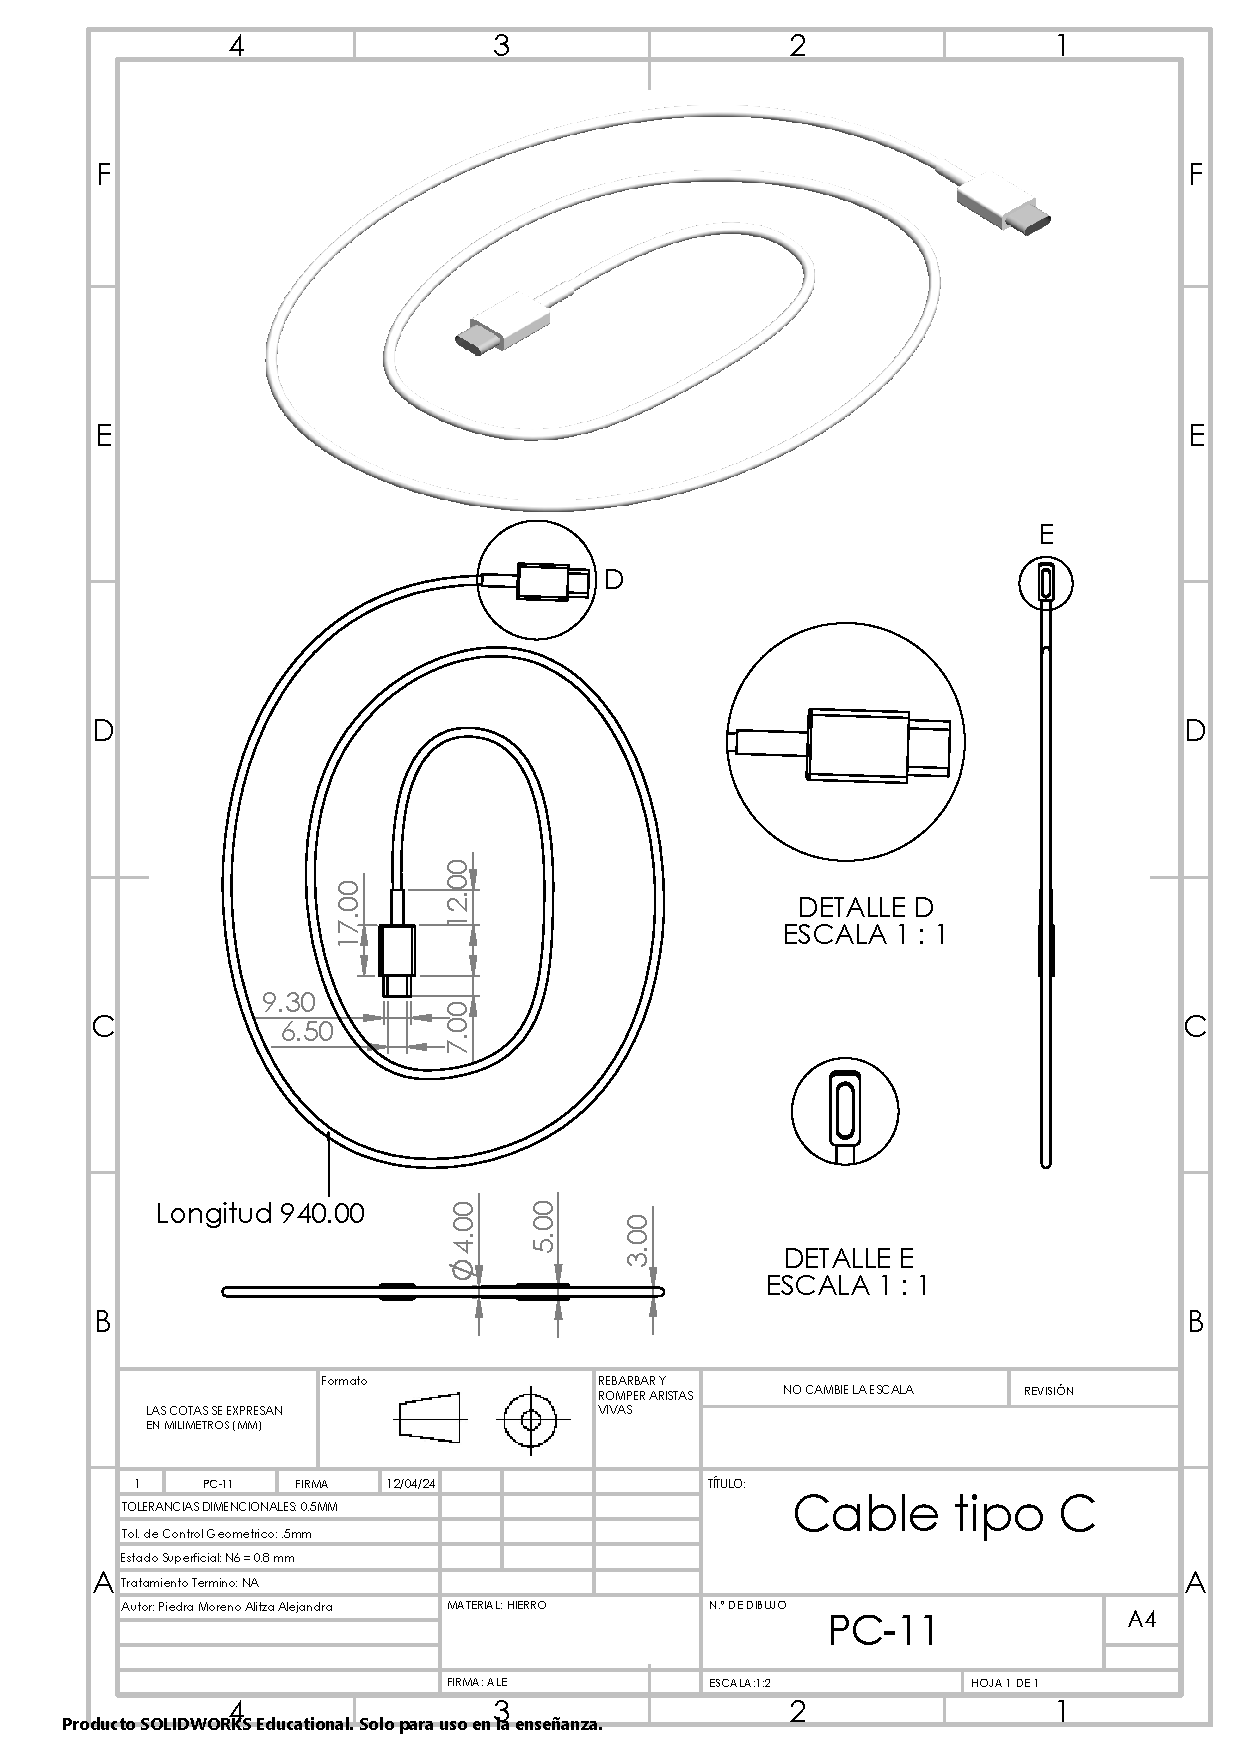
\includegraphics[trim = {7mm 1mm 1mm 1mm},clip,scale=0.4]{22/Img/cableCDibujo.PDF}
    \caption{Dibujo técnico: Cable MM}
    \label{fig:enter-label9}
\end{figure}



\subsection{Desarrollo}

Cada estrategia metodológica se establece acorde a cada objetivo, y por tanto deberá ser desglosada precisada y ordenada claramente. En consecuencia cada objetivo que se presentó en forma de verbo en infinitivo deberá determinar una estrategia en forma de adverbio. Ej. Desarrollar…Desarrollo. Son las actividades ordenadas que tienen como finalidad la prueba de la hipótesis. 

\begin{itemize}
    \item Se debe establecer que se habrá de hacer, como, conque, y donde para obtener la información que permita probar la hipótesis.  
    \item Se debe desglosar de acuerdo a los objetivos específicos. 
    \item Se debe establecer una estrategia metodológica por cada objetivo específico. De manera simplista se podría decir que se cambia el verbo en infinitivo por su respectivo adverbio.
    \item En cada objetivo se debe describir que método, que materiales y que equipo se usará para conseguirlo.
    \item Se deben tener referencias Figura \ref{fig:lcd-16x2}.
\end{itemize}
% 
% 

% 
% 
\subsection{Prepara tu documento}

Antes de que comiences a utilizar esta plantilla, es recomendable que prepare la información que contendrá en un archivo aparte. 
Ten preparadas tus gráficas, así como también las tablas aparte, para que sea más fácil integrarlo. 
Se recomienda fuertemente el uso de \textbf{formato Enhanced Metafile (.emf) para imágenes y gráficas} de resolución óptima. 
Finalmente, completa y organiza el contenido antes de darle el formato de esta plantilla. 

\subsection{Acrónimos y Abreviaciones}

Los acrónimos y abreviaciones deberán ser definidos únicamente la primera vez que aparecen en el texto, esto para que el lector entienda lo que significan.

\subsection{Ecuaciones}

Las ecuaciones son una excepción a las especificaciones prescritas de esta plantilla. 
Deberá determinar si su ecuación debe escribirse o no utilizando la fuente Adobe Devangari. 
Para crear ecuaciones multinivel, puede ser necesario tratar la ecuación como un gráfico e insertarla en el texto después de aplicar el estilo de la platilla.
Las ecuaciones serán enumeradas de manera consecutiva, y el número de ecuación, entre paréntesis, se colocan al ras de la derecha, utilizando una tabulación derecha. 

\begin{equation}
    \label{eq1}
    x + y = z 
\end{equation}

Es importante asegurarse de que los símbolos de la ecuación sean definidos antes o inmediatamente después de la ecuación. Utilice “(1)”, en vez de “Eq. 1” al enumerar las ecuaciones, excepto al principio de una oración: “La ecuación (\ref{eq1}) es…”

\section{Resultados y discusión}

Antes de comenzar a preparar tu artículo, es importante que lea primero la guía del autor, la cual incluye los temas o apartados que son necesarios para tener tu trabajo completo.
Una vez completada la edición del texto, el documento está listo para el uso de esta plantilla. En este archivo recién creado, resalte todo el contenido e importe el archivo de texto preparado. Ahora esta listo para estilizar su documento.
En esta sección se deben presentar todo lo obtenido de la sección 2, incluidas deducciones o efectos del desarrollo. También se podrán incluir subsecciones numeradas de la siguiente forma:

\subsection{Autores y Afiliaciones}

Para distinguir las afiliaciones de los autores, utilice superíndices iniciando con el número 1, 2, etc., sucesivamente, esto dependerá de la cantidad de los departamentos a los que estén afiliados los autores. En caso de que todos los autores pertenezcan a una mismo departamento e institución, utilizar sólo el superíndice 1. 

\subsection{Identificar los encabezados}

Se les recuerda a los autores que los encabezados deben de estar conforme los solicita la guía del autor. De ahí se puede adaptar el trabajo para que sea más fácil de entender para el lector.
Los encabezados organizan los temas sobre una base relacional y jerárquica. Por ejemplo, el título del documento es encabezado del texto principal porque todo el material posterior se relaciona y elabora sobre este tema. 

\subsection{Tablas y Figuras}

\begin{enumerate}
    \item Posición de las tablas y figuras: Coloque las figuras y las tablas en la parte superior e inferior de las columnas. Evite colocarlos en medio. Las figuras y las tablas grandes pueden abarcar ambas columnas. Los títulos de las figuras deben de estar debajo de las mismas; los títulos de las tablas deben aparecer encima de ellas. Insértese las figuras y los cuadros después de citarse en el texto. Utilice la abreviatura “Fig. 1”, incluso al principio de una oración. 
\end{enumerate}

\section{Conclusiones}

Se describe aquí el alcance del trabajo, logros obtenidos y perspectivas para el futuro de este. Se sugiere colocar información cuantitativa obtenida.

\section{Agradecimientos}

Es importante darles su debido reconocimiento a los laboratorios, instituciones, organizaciones, entre otros que han sido partícipes para la culminación de este trabajo. También es importante mencionar, fondos, proyectos, becas, entre otros que se le han otorgado al o los autores para realizar el trabajo de investigación. Ejemplo: “Los autores agradecen al Concejo Nacional de Ciencia y Tecnología por los recursos otorgados…”

\section*{Referencias}

Para esta platilla, se solicita al autor enumerar las citas de manera consecutiva entre corchetes \cite{YLi2013}. 
La puntuación de la oración que sigues sería \cite{Mesaelides2011}. 
Refiérase simplemente al número de referencia, como en \cite{Morales2012}, no utilice “Ref. [3]” o “referencia [3]” excepto al principio de una oración: “La referencia [3] fue la primera…”
Enumere las notas al pie por separado en superíndices. Coloque la nota de pie de en la parte inferior de la columna en la que se citó. No coloque notas al pie en la lista de referencias. Utilice letras para las notas al pie de la tabla.
A menos de que haya tres autores o más; no utilice “et al.”. Los trabajos que no hayan sido publicados, incluso si han sido presentados para su publicación, deben ser citados como “inéditos”. Los trabajos que han sido aceptados para su publicación deben de citarse como “en prensa”. Poner en mayúscula solo la primera palabra de un título, excepto los nombres propios y los símbolos de elemento. 
Otros ejemplos \cite{LAAngeles2021}, \cite{LAAngelesConni}. 
Véase el archivo adjunto \ref{Figura:instructivo}


% \newpage
% \bibliographystyle{ieeetr}
% \bibliography{22/referencias}
% 
% 
%%%%%%%%%%%%%%%%%%%%%%%%%%%%%%%%%%
\appendix
%%%%%%%%%%%%%%%%%%%%%%%%%%%%%%%%%%
% 
\centering{\section[\appendixautorefname{}]{Apéndice Instructivo}}\label{Figura:instructivo}
\includepdf[pages=3-5 ]{22/Img/instructivoMateriales.pdf}
%%%%%%%%%%%%%%%%%%%%%%%%%%%%%%%%%%%%%%%%
% 
\centering{\section[\appendixautorefname{}]{Apéndice Materiales}}\label{Figura:Materiales}
\includepdf[page=6-8,]{22/Img/instructivoMateriales.pdf}
% 
%%%%%%%%%%%%%%%%%%%%%%%%%%%%%%%%%%%%%%%%
\centering{\section[\appendixautorefname{}]{Apéndice de Formato}}\label{Figura:Hoja de datos}
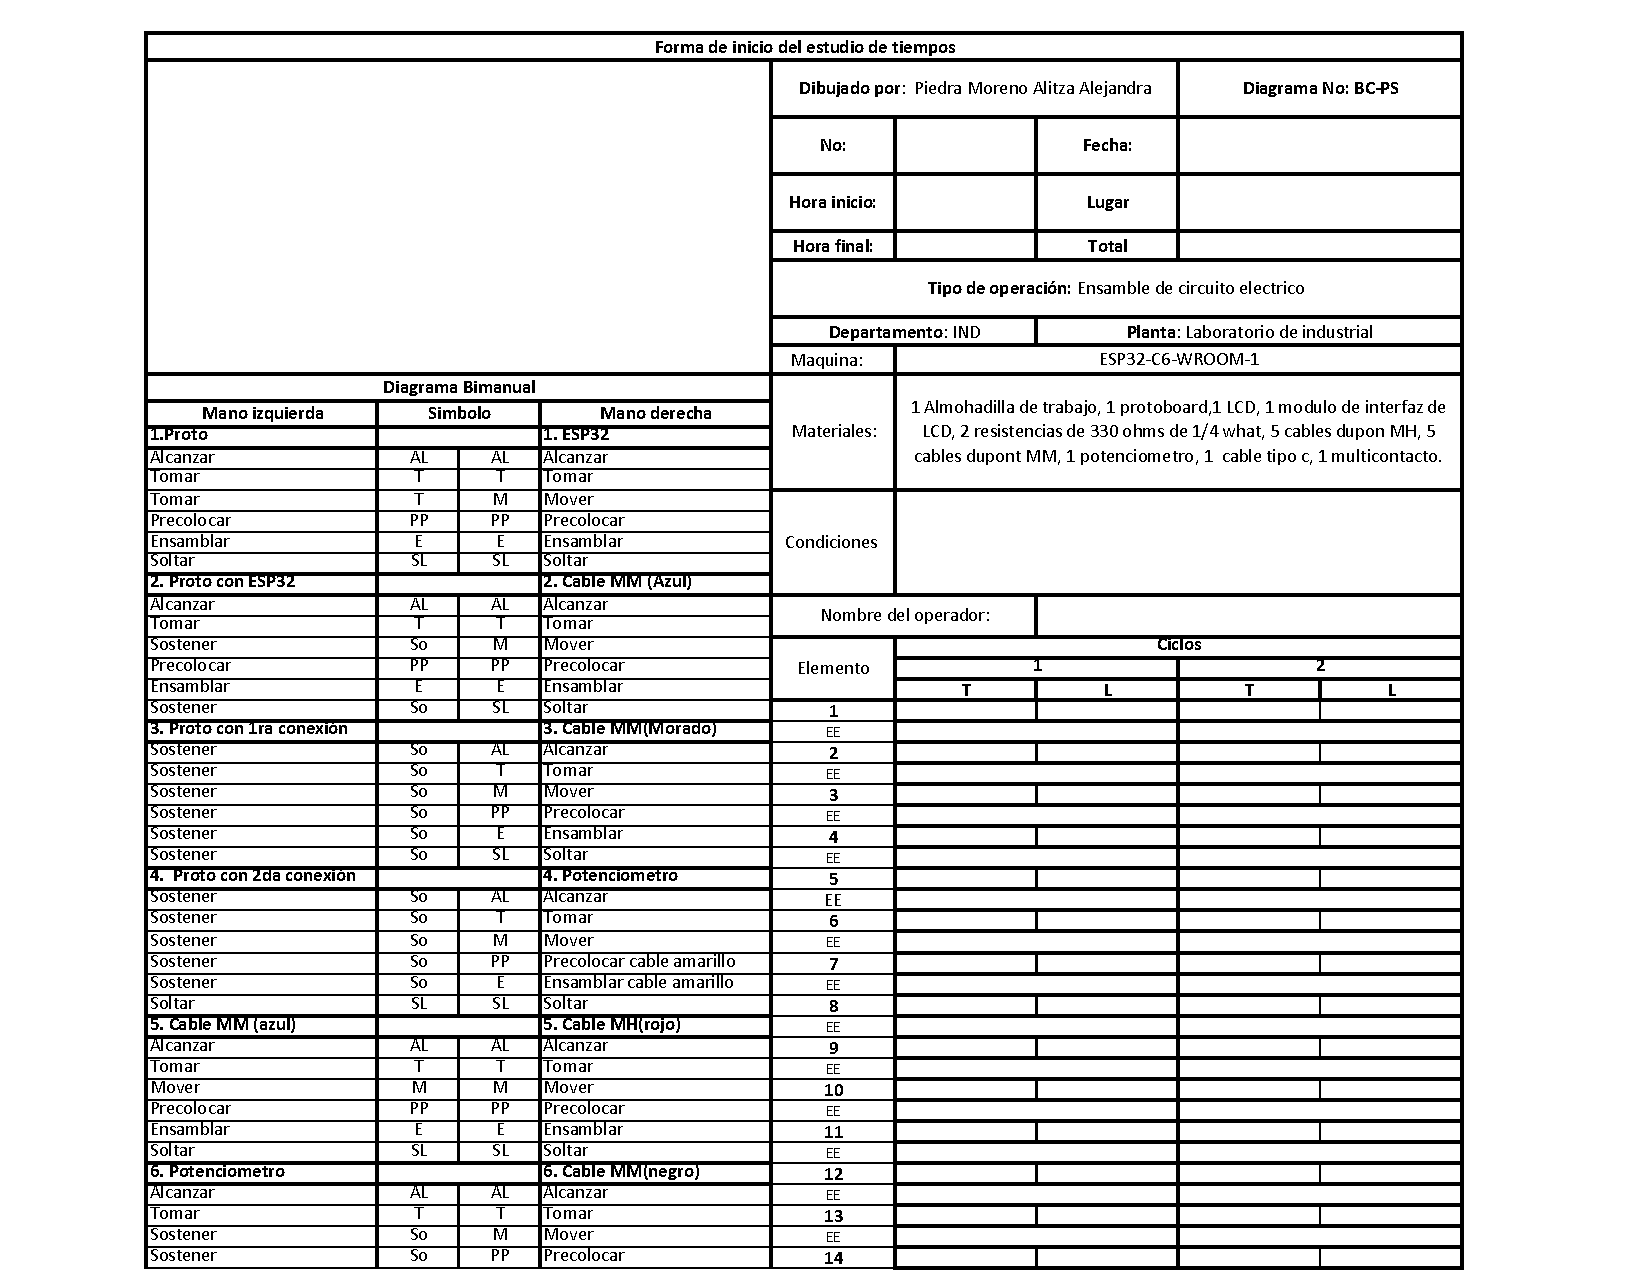
\includepdf[page=-,]{22/Img/Formato.pdf}


\newpage
\bibliographystyle{ieeetr}
\bibliography{22/referencias}